% Options for packages loaded elsewhere
\PassOptionsToPackage{unicode}{hyperref}
\PassOptionsToPackage{hyphens}{url}
%
\documentclass[
  12pt,
]{article}
\usepackage{lmodern}
\usepackage{amssymb,amsmath}
\usepackage{ifxetex,ifluatex}
\ifnum 0\ifxetex 1\fi\ifluatex 1\fi=0 % if pdftex
  \usepackage[T1]{fontenc}
  \usepackage[utf8]{inputenc}
  \usepackage{textcomp} % provide euro and other symbols
\else % if luatex or xetex
  \usepackage{unicode-math}
  \defaultfontfeatures{Scale=MatchLowercase}
  \defaultfontfeatures[\rmfamily]{Ligatures=TeX,Scale=1}
\fi
% Use upquote if available, for straight quotes in verbatim environments
\IfFileExists{upquote.sty}{\usepackage{upquote}}{}
\IfFileExists{microtype.sty}{% use microtype if available
  \usepackage[]{microtype}
  \UseMicrotypeSet[protrusion]{basicmath} % disable protrusion for tt fonts
}{}
\makeatletter
\@ifundefined{KOMAClassName}{% if non-KOMA class
  \IfFileExists{parskip.sty}{%
    \usepackage{parskip}
  }{% else
    \setlength{\parindent}{0pt}
    \setlength{\parskip}{6pt plus 2pt minus 1pt}}
}{% if KOMA class
  \KOMAoptions{parskip=half}}
\makeatother
\usepackage{xcolor}
\IfFileExists{xurl.sty}{\usepackage{xurl}}{} % add URL line breaks if available
\IfFileExists{bookmark.sty}{\usepackage{bookmark}}{\usepackage{hyperref}}
\hypersetup{
  hidelinks,
  pdfcreator={LaTeX via pandoc}}
\urlstyle{same} % disable monospaced font for URLs
\usepackage[margin=1in]{geometry}
\usepackage{graphicx}
\makeatletter
\def\maxwidth{\ifdim\Gin@nat@width>\linewidth\linewidth\else\Gin@nat@width\fi}
\def\maxheight{\ifdim\Gin@nat@height>\textheight\textheight\else\Gin@nat@height\fi}
\makeatother
% Scale images if necessary, so that they will not overflow the page
% margins by default, and it is still possible to overwrite the defaults
% using explicit options in \includegraphics[width, height, ...]{}
\setkeys{Gin}{width=\maxwidth,height=\maxheight,keepaspectratio}
% Set default figure placement to htbp
\makeatletter
\def\fps@figure{htbp}
\makeatother
\setlength{\emergencystretch}{3em} % prevent overfull lines
\providecommand{\tightlist}{%
  \setlength{\itemsep}{0pt}\setlength{\parskip}{0pt}}
\setcounter{secnumdepth}{-\maxdimen} % remove section numbering
\usepackage{booktabs}
\usepackage{longtable}
\usepackage{array}
\usepackage{multirow}
\usepackage{wrapfig}
\usepackage{float}
\usepackage{colortbl}
\usepackage{pdflscape}
\usepackage{tabu}
\usepackage{threeparttable}
\usepackage{threeparttablex}
\usepackage[normalem]{ulem}
\usepackage{makecell}
\usepackage{caption}
\usepackage{hyperref}
\usepackage{helvet} % Helvetica font
\renewcommand*\familydefault{\sfdefault} % Use the sans serif version of the font
\usepackage[T1]{fontenc}
\usepackage[labelfont=bf]{caption}

\usepackage[none]{hyphenat}

\usepackage{setspace}
\doublespacing
\setlength{\parskip}{1em}

\usepackage{lineno}

\usepackage{pdfpages}
\floatplacement{figure}{H} % Keep the figure up top of the page
\DeclareUnicodeCharacter{0301}{*************************************}
\newlength{\cslhangindent}
\setlength{\cslhangindent}{1.5em}
\newenvironment{cslreferences}%
  {}%
  {\par}

\author{}
\date{\vspace{-2.5em}}

\begin{document}

\pagenumbering{arabic}
\linenumbers
\doublespacing

\hypertarget{the-gut-bacterial-community-potentiates-clostridioides-difficile-infection-severity.}{%
\section{\texorpdfstring{The gut bacterial community potentiates
\emph{Clostridioides difficile} infection
severity.}{The gut bacterial community potentiates Clostridioides difficile infection severity.}}\label{the-gut-bacterial-community-potentiates-clostridioides-difficile-infection-severity.}}

\vspace{30mm}

\textbf{Running title:} Microbiota potentiates \emph{Clostridioides
difficile} infection severity

\vspace{20mm}

Nicholas A. Lesniak\(^1\), Alyxandria M. Schubert\(^1\), Kaitlyn J.
Flynn\(^1\), Jhansi L. Leslie\(^{1,4}\), Hamide Sinani\(^1\), Ingrid L.
Bergin\(^3\), Vincent B. Young\(^{1,2}\), Patrick D.
Schloss\(^{1,\dagger}\)

\vspace{30mm}

\(\dagger\) To whom correspondence should be addressed:
\href{mailto:pschloss@umich.edu}{\nolinkurl{pschloss@umich.edu}}\\
1. Department of Microbiology and Immunology, University of Michigan,
Ann Arbor, MI\\
2. Division of Infectious Diseases, Department of Internal Medicine,
University of Michigan Medical School, Ann Arbor, MI\\
3. Unit for Laboratory Animal Medicine, University of Michigan, Ann
Arbor, MI\\
4. Current affiliation: Department of Medicine, Division of
International Health and Infectious Diseases, University of Virginia
School of Medicine, Charlottesville, Virginia, USA

\newpage

\hypertarget{abstract}{%
\subsection{Abstract}\label{abstract}}

The severity of \emph{Clostridioides difficile} infections (CDI) has
increased over the last few decades. Patient age, white blood cell
count, creatinine levels as well as \emph{C. difficile} ribotype and
toxin genes have been associated with disease severity. However, it is
unclear whether there is an association between the gut microbiota and
disease severity. The gut microbiota is known to interact with \emph{C.
difficile} during infection. Perturbations to the gut microbiota are
necessary for \emph{C. difficile} to colonize the gut. The gut
microbiota is thought to impair \emph{C. difficile} colonization through
bile acid metabolism, nutrient consumption and bacteriocin production.
Here we sought to demonstrate that members of the gut bacterial
communities can contribute to disease severity. We derived diverse gut
communities by colonizing germ-free mice with different human fecal
communities. The mice were then infected with a single \emph{C.
difficile} ribotype 027 clinical isolate which resulted in moribundity
and histopathologic differences. The variation in severity was
associated with the human fecal community that the mice received.
Generally, bacterial populations with pathogenic potential, such as
\emph{Escherichia}, \emph{Helicobacter}, and \emph{Klebsiella}, were
associated with more severe outcomes. Bacterial groups associated with
fiber degradation, bile acid metabolism and lantibiotic production, such
as \emph{Anaerostipes} and \emph{Coprobacillus}, were associated with
less severe outcomes. These data indicate that gut bacteria can
influence CDI disease severity.

\hypertarget{importance}{%
\subsection{Importance}\label{importance}}

\emph{Clostridioides difficile} colonization can result in no symptoms
or develop into an infection, ranging in severity from mild diarrhea to
toxic megacolon, sepsis and death. Models that predict severity and
guide treatment decisions are based on clinical factors and \emph{C.
difficile} characteristics. Although the gut microbiome plays a role in
protecting against CDI, it has not been investigated for its effect on
CDI disease severity or incorporated into attempts to predict disease
severity. We demonstrated that variation in the microbiome of mice
colonized with human feces yielded a range of disease outcomes. These
results revealed groups of bacteria associated with both severe and mild
\emph{C. difficile} infection outcomes. Gut bacterial community data
from patients with CDI could improve our ability to identify patients at
risk of developing more severe disease and improve interventions which
target \emph{C. difficile} and the gut bacteria to reduce host damage.

\newpage

\hypertarget{introduction}{%
\subsection{Introduction}\label{introduction}}

\emph{Clostridioides difficile} infections (CDI) have increased in
incidence and severity since \emph{C. difficile} was first identified as
the cause of antibiotic-associated pseudomembranous colitis (1). CDI
disease severity can range from asymptomatic to mild diarrhea to toxic
megacolon and death. The Infectious Diseases Society of America (IDSA)
and Society for Healthcare Epidemiology of America (SHEA) guidelines
defines severe CDI in terms of a white blood cell count greater than
15,000 cells/mm\(^3\) and/or a serum creatinine greater than 1.5 mg/dL.
Patients who develop shock or hypotension, ileus, or toxic megacolon are
considered to have fulminant CDI (2). Since these measures are outcomes
of CDI, these measures have limited ablity to predict risk of severe CDI
when CDI is fiest detected. Schemes have been developed to score a
patient's risk for severe CDI outcomes based on clinical factors but
have not been robust for broad application (3). Thus, we have limited
ability to prevent patients from developing severe CDI. Ideally, we
could identify patients that are high-risk of severe disease so their
treatments could be adjusted to alter the clinical trajectory.

Missing from CDI severity prediction models are the effects of the
indigenous gut bacteria. \emph{C. difficile} interacts with the gut
community in many ways. The indigenous bacteria of a healthy intestinal
community provide a protective barrier preventing \emph{C. difficile}
from infecting the gut. A range of mechanisms can disrupt this barrier,
including antibiotics, medications, or dietary changes, and lead to
increased susceptibility to CDI (4--6). Once \emph{C. difficile}
overcomes the protective barrier and colonizes the intestine, the
indigenous bacteria can either promote or inhibit \emph{C. difficile}
through producing molecules or modifying the environment (7, 8). Bile
acids metabolized by the gut bacteria can inhibit \emph{C. difficile}
growth and affect toxin production (9, 10). Bacteria in the gut also can
compete more directly with \emph{C. difficile} through antibiotic
production or nutrient consumption (11--13). While the relationship
between the gut bacteria and \emph{C. difficile} has been established,
the effect the gut bacteria can have on CDI disease severity is unclear.

Here, we sought to determine whether the gut bacteria contribute to
disease severity. We hypothesized that since the gut bacteria affect the
metabolism of \emph{C. difficile} and its infection dynamics, it can
also affect the disease severity of the infection. To test this
hypothesis, we colonized germ-free C57BL/6 mice with human fecal samples
to create varied gut communities. We then challenged the mice with a
single \emph{C. difficile} isolate, ribotype 027 (RT027) clinical
isolate 431, and followed the mice for the development of severe
outcomes of moribundity and histopathologic cecal tissue damage. Since
the murine host and \emph{C. difficile} isolate were the same and only
the gut community varied, the variation in disease severity we observed
was attributable to the microbiome.

\hypertarget{results}{%
\subsection{Results}\label{results}}

\textbf{\emph{C. difficile} is able to infect germ-free mice colonized
with human fecal microbial communities without antibiotics} To produce
gut microbiomes with greater variation than those found in conventional
mouse colonies, we colonized germ-free mice with bacteria from human
feces (14). We inoculated germ-free C57BL/6 mice with homogenized feces
from one of 15 human fecal samples via oral gavage. These human fecal
samples were selected because they represented diverse community
structures based on community clustering (15). The gut communities were
allowed to equlibriate for two weeks post inoculation (16). We then
surveyed the bacterial members of the gut communities by 16S rRNA gene
sequencing of murine fecal pellets (Figure 1A). The bacterial
communities from each mouse grouped more closely to those communities
from mice that received the same human fecal donor community than to the
mice who received a different human fecal donor community (Figure 1B).
The communities were primarily composed of populations of
\emph{Clostridia}, \emph{Bacteroidia}, \emph{Erysipelotrichia},
\emph{Bacilli}, and \emph{Gammaproteobacteria}. However, the gut
bacterial communities of each donor group of mice harbored unique
relative abundance distributions of the shared bacterial classes.

Next, we tested this set of mice with their human-derived gut microbial
communities for susceptibility to \emph{C. difficile} infection. A
typical mouse model of CDI requires pre-treatment of conventional mice
with antibiotics, such as clindamycin, to become susceptible to \emph{C.
difficile} colonization (17, 18). However, we wanted to avoid modifying
the gut communities with an antibiotic to maintain their unique
microbial compositions and ecological relationships. Since some of these
communities came from people at increased risk of CDI, for example due
to hospitalization or recent antibiotic use (15), we decided to test if
\emph{C. difficile} was able to infect these mice without any antibiotic
perturbation. We hypothesized that \emph{C. difficile} would be able to
colonize the mice who received their gut communities from a donor with
perturbed community. Mice were challenged with 10\(^{3}\) \emph{C.
difficile} RT027 clinical isolate 431 spores. The mice were followed for
10 days post-challenge, and their stool was collected and plated for
\emph{C. difficile} colony forming units (CFU) to determine the extent
of the infection. Surprisingly, communities from all donors were able to
be colonized (Figure 2). Two mice were able to resist \emph{C.
difficile} colonization, both received their community donor N3, which
may be attributed to experimental variation since this group also had
more mice. By colonizing germ-free mice with different human fecal
communities, we were able to generate diverse gut communities in mice,
which were susceptible to \emph{C. difficile} infection without further
modification of the gut community.

\textbf{Infection severity varies by initial community.} After we
challenged the mice with \emph{C. difficile}, we investigated the
outcome from the infection and its relationship to the initial
community. We followed the mice for 10 days post-challenge for
colonization density, toxin production, and mortality. Seven mice, from
Donors N1, N2 and N5, were not colonized at detectable levels on the day
after \emph{C. difficile} challenge but were infected
(\textgreater10\(^{6}\)) by the end of the experiment. All mice that
received their community from Donor M1 through M6 succumbed to the
infection and became moribund within 3 days post-challenge. The
remaining mice, except the uninfected Donor N3 mice, maintained \emph{C.
difficile} infection through the end of the experiment (Figure 2). At 10
days post-challenge, or earlier for the moribund mice, mice were
euthanised and fecal material were assayed for toxin activity and cecal
tissue was collected and scored for histopathologic signs of disease
(Figure 3). Overall, there was greater toxin activity detected in the
stool of the moribund mice (\emph{P} = 0.003). However, when looking at
each group of mice, we observed a range in toxin activity for both the
moribund and non-moribund mice (Figure 3A). Non-moribund mice from
Donors N4 through N9 had comparable toxin activity as the moribund mice.
Additionally, not all moribund mice had toxin activity detected in their
stool. Next we examined the cecal tissue for histopathologic damage.
Moribund mice had high levels of epithelial damage, tissue edema, and
inflammation (Figure S1) similar to previously reported histopathologic
findings for \emph{C. difficile} RT027 (19). As observed with toxin
activity, the moribund mice had higher histopathologic scores than the
non-moribund mice (\emph{P} \textless{} 0.001). However, unlike the
toxin activity, all moribund mice had consistently high histopathologic
summary scores (Figure 3B). The non-moribund mice, Donor groups N1
through N9, had a range in tissue damage from none detected to similar
levels as the moribund mice, which grouped by community donor. Together,
the toxin activity, histopathologic score, and moribundity showed
variation across the donor groups but were largely consistent within
each donor group.

\textbf{Microbial community members explain variation in CDI severity.}
We next interrogated the bacterial communities at the time of \emph{C.
difficile} challenge (day 0) for their relationship to infection
outcomes using linear discriminant analysis (LDA) effect size (LEfSe)
analysis to identify individual bacterial populations that could explain
the variation in disease severity. We split the mice into groups by
severity level based on their moribundity and histopathologic score. We
dichotomized the histopathologic scores into high and low groups by
splitting on the median score of 5. This analysis revealed 20 genera
that were significantly different by the disease severity (Figure 4A).
Bacterial genera \emph{Turicibacter}, \emph{Streptococcus},
\emph{Staphylococcus}, \emph{Pseudomonas}, \emph{Phocaeicola},
\emph{Parabacteroides}, \emph{Bacteroides}, and
\emph{Escherichia/Shigella} were detected at higher relative abundances
in the mice that became moribund. Populations of \emph{Anaerotignum},
\emph{Coprobacillus}, \emph{Enterocloster}, and \emph{Murimonas} were
more abundant in the non-moribund mice that would develop only low
intestinal injury. To understand the role of toxin activity in disease
severity, we applied LEfSe to identify the genera most likely to explain
the differences between the presence and absence of detected toxin
activity (Figure 4B). Many genera that associated with toxin production
were also associated with moribundity, such as populations of
\emph{Escherichia/Shigella} and \emph{Bacteroides}. Likewise, there were
genera such as \emph{Anaerotignum}, \emph{Enterocloster}, and
\emph{Murimonas} that were associated with no detected toxin production
that also exhibited greater relative abundance in communities from
non-moribund mice with a low histopathologic score. Lastly, we tested
for correlations between the endpoint relative abundances of bacterial
operational taxonomic units (OTUs) and the histopathologic summary score
(Figure 4C). The endpoint relative abundance of \emph{Bacteroides} was
positively correlated with histopathologic score, as its day 0 relative
abundance did with disease severity (Figure 4A). Populations of
\emph{Klebsiella} and \emph{Prevotellaceae} were positively correlated
with the histopathologic score and were increased in the group of mice
with detectable toxin. This analysis identified bacterial genera that
were associated with the variation in moribundity, histopathologic
score, and toxin activity of CDI.

We next determined whether collectively, bacterial community membership
and relative abundance could be predictive of the CDI disease outcome.
We trained random forest models with bacterial community relative
abundance data from the day of colonization at each taxonomic rank to
predict toxin production, moribundity, and day 10 post-challenge
histopathologic summary score. For predicting if toxin would be
produced, microbial populations aggregated by phylum rank classification
performed similarly as models using lower taxonomic ranks (AUROC = 0.83,
Figure S2). \emph{C. difficile} was more likely to produce toxin when
the community it infected had less abundant populations of
\emph{Verrucomicrobia} and \emph{Campilobacterota} and had more abundant
populations of \emph{Proteobacteria} (Figure 5A). Next, we assessed the
ability of the community to predict moribundity. Bacteria grouped by
class rank classification was sufficient to predict which mice would
succumb to the infection before the end of the experiment (AUROC = 0.91,
Figure S2). The features with the greatest effect showed that
communities with greater populations of bacteria belonging to
\emph{Bacilli} and \emph{Firmicutes} and reduced populations of
\emph{Erysipelotrichia} were more likely to result in moribundity
(Figure 5B). Only one other class of bacteria was decreased in moribund
mice, a group of unclassified \emph{Clostridia}. Lastly, the relative
abundances of genera were able to predict a high or low histopathologic
score (histopathologic scores were dichotomized as in previous analysis,
AUROC = 0.99, Figure S2). No genera had a significantly greater effect
on the model performance than any others, indicating the model was
reliant on many genera for the correct prediction. The model used some
of the genera identified in the LEfSe analysis, such as
\emph{Coprobacillus}, \emph{Anaerostipes}, and \emph{Hungatella}.
Communities with greater abundances of \emph{Hungatella},
\emph{Eggerthella}, \emph{Bifidobacterium}, \emph{Duncaniella} and
\emph{Neisseria} were more likely to have high histopathologic scores.
These models have shown that the relative abundance of bacterial
populations and their relationship to each other could be used to
predict the variation in moribundity, histopathologic score, and toxin
activity of CDI.

\hypertarget{discussion}{%
\subsection{Discussion}\label{discussion}}

Challenging mice colonized with different human fecal communities with a
single \emph{C. difficile} isolate, RT027 isolate 431, demonstrated that
variation in the gut bacteria affects the \emph{C. difficile} infection
disease severity. Our analysis revealed an association between the
relative abundance of bacterial community members and disease severity.
Previous studies investigating the severity of CDI disease involving the
microbiome have had limited ability to interrogate this relationship
between the microbiome and disease severity. Studies that have used
clinical data have limited ability to control variation in the host,
microbiome or \emph{C. difficile} ribotype (20). Murine experiments
typically use a single mouse colony and different \emph{C. difficile}
ribotypes to create severity differences (21). Recently, our group has
begun uncovering the effect microbiome variation has on \emph{C.
difficile} infection. We showed the variation in the bacterial
communities between mice from different mouse colonies resulted in
different clearance rates of \emph{C. difficile} (22). We also showed
varied ability of mice to spontaneously eliminate \emph{C. difficile}
infection when they were treated with different antibiotics prior to
\emph{C. difficile} challenge (23). Overall, the results presented here
have demonstrated that the gut bacterial community contributed to the
severity of \emph{C. difficile} infection.

\emph{C. difficile} can lead to asymptomatic colonization or infections
with severity ranging from mild diarrhea to death. Physicians use
classification tools to identify patients most at risk of developing a
severe infection using white blood cell counts, serum albumin level, or
serum creatinine level (2, 24, 25). Those levels are driven by the
activities in the intestine (26). Research into the drivers of this
variation have revealed factors that make \emph{C. difficile} more
virulent. Strains are categorized for their virulence by the presence
and production of the toxins TcdA, TcdB, and binary toxin and the
prevalence in outbreaks, such as ribotypes 027 and 078 (17, 27--30).
However, other studies have shown that disease is not necessarily linked
with toxin production (31) or the strain (32). Furthermore, there is
variation in the genome, growth rate, sporulation, germination, and
toxin production in different isolates of a strain (33--36). This
variation may help explain why severe CDI prediction tools often miss
identifying many patients with CDI that will develop severe disease (3,
21, 37, 38). Therefore, it is necessary to gain a full understanding of
all factors contributing to disease variation to improve our ability to
predict severity.

The state of the gut bacterial community determines the ability of
\emph{C. difficile} to colonize and persist in the intestine. \emph{C.
difficile} is unable to colonize an unperturbed healthy gut community
and is only able to become established after a perturbation (18). Once
colonized, the different communities lead to different metabolic
responses and dynamics of the \emph{C. difficile} population (8, 23,
39). Gut bacteria metabolize primary bile acids into secondary bile
acids (40, 41). The concentration of these bile acids affects
germination, growth, toxin production and biofilm formation (9, 10, 42,
43). Members of the bacterial community also affect other metabolites
\emph{C. difficile} utilizes. \emph{Bacteroides thetaiotaomicron}
produce sialidases which release sialic acid from the mucosa for
\emph{C. difficile} to utilize (44, 45). The nutrient environment
affects toxin production (46). Thus, many of the actions of the gut
bacteria modulate \emph{C. difficile} in ways that could affect the
infection and resultant disease.

A myriad of studies have explored the relationship between the
microbiome and CDI disease. CDI studies often use an infection model
with a single homogeneous bacterial community. Collins \emph{et al.}
used multiple human communities to colonize mice, however the
communities were pooled prior to gavaging into germ-free mice (47),
resulting in a single human-derived community. Studies examining
difference in disease often use different \emph{C. difficile} strains or
ribotypes in mice with similar microbiota as a proxy for variation in
disease, such as strain 630 for non-severe and RT027 for severe (17, 27,
28, 48). Studies have also demonstrated variation in infection through
tapering antibiotic dosage (18, 23, 49) or by reducing the amount of
\emph{C. difficile} cells or spores used for the challenge (17, 49).
These studies either lack variation in the initial microbiome or have
variation in the \emph{C. difficile} infection itself, confounding any
association between variation in severity and the microbiome.
\textbf{Add Hikiro et al} With our recent observations that the initial
community affected the ability of \emph{C. difficile} to persist in the
gut (22, 23) and the existing research describing the numerous
interactions between the microbiome and \emph{C. difficile}, we
hypothesized that the microbiome can modulate CDI disease severity. Our
data have demonstrated gut bacterial relative abundances associate with
variation in toxin production, histopathologic scoring of the cecal
tissue and mortality. This analysis revealed populations of
\emph{Akkermansia}, \emph{Anaerostipes}, \emph{Coprobacillus},
\emph{Enterocloster}, \emph{Lactonifactor}, and \emph{Monoglobus} were
more abundant in the microbiome of non-moribund mice which had low
histopathologic scores and no detected toxin. The protective role of
these genera are supported by previous studies. \emph{Coprobacillus},
\emph{Lactonifactor}, and \emph{Monoglobus} have been shown to be
involved in dietary fiber fermentation and associated with healthy
communities (50--53). \emph{Anaerostipes} and \emph{Coprobacillus},
which produce short chain fatty acids, have been associated with healthy
communities (54--56). Furthermore, \emph{Coprobacillus}, which was
abundant in mice with low histopathologic scores but rare in all other
mice, has been shown to contain a putative type I lantibiotic gene
cluster and inhibit \emph{C. difficile} colonization (57--59).
\emph{Akkermansia} and \emph{Enterocloster} were also identified as more
abundant in mice which had a low histopathologic scores but have
contradictory supporting evidence in the current literature. In our
data, \emph{Akkermansia} was most abundant in the non-moribund mice with
low histopathologic scores but there were some moribund mice which had
increased populations of \emph{Akkermansia}. This could be attributed to
either a more protective mucus layer was present inhibiting colonization
(59, 60) or mucus consumption by \emph{Akkermansia} could have been
crossfeeding \emph{C. difficile} or exposing a niche for \emph{C.
difficile} (61--63). Similarly, \emph{Enterocloster} was more abundant
and associated with low histopathologic scores. It has been associated
with healthy populations and has been used to mono-colonize germ-free
mice to reduce the ability of \emph{C. difficile} to colonize (64, 65).
However, \emph{Enterocloster} has also been involved in infections, such
as bacteremia (66, 67). These data have exemplified populations of
bacteria that have the potential to be either protective or harmful.
Thus, the disease outcome is not likely based on the abundance of
individual populations of bacteria, rather it is the result of the
interactions of the community.

The groups of bacteria that were associated with either a higher
histopathologic score or moribundity are members of the indigenous gut
community that also have been associated with disease, often referred to
as opportunistic pathogens. Many of the populations with pathogenic
potential that associated with worse outcomes are also facultative
anaerobes. \emph{Enterococcus}, \emph{Klebsiella},
\emph{Shigella/Escherichia}, \emph{Staphylococcus}, and
\emph{Streptococcus} have been shown to expand after antibiotic use (15,
68, 69) and are commonly detected in CDI cases (70--73). In addition to
these populations, \emph{Eggerthella}, \emph{Prevotellaceae} and
\emph{Helicobacter}, which associated with worse outcomes, have also
been associated with intestinal inflammation (74--76). Recently,
\emph{Helicobacter hepaticus} was shown to be sufficient to cause
susceptibility to CDI in IL-10 deficient C57BL/6 mice (77). In our
experiments, when \emph{Helicobacter} was present, the infection
resulted in a high histopathologic score (Figure 4C). While we did not
use IL-10 deficient mice, it is possible the bacterial community or host
response are similarly modified by \emph{Helicobacter}, allowing
\emph{C. difficile} infection and host damage. Aside from
\emph{Helicobacter}, these groups of bacteria that associated with more
severe outcomes did not have a conserved association between their
relative abundance and the disease severity across all mice.

Since we observed groups of bacteria that were associated with less
severe disease it may be appropriate to apply the damage-response
framework for microbial pathogenesis to CDI (78, 79). This framework
posits that disease is not driven by a single entity, rather it is an
emergent property of the responses of the host immune system, infecting
microbe, \emph{C. difficile}, and the indigenous microbes at the site of
infection. In the first set of experiments, we used the same host
background, C57BL/6 mice, the same infecting microbe, \emph{C.
difficile} RT027 clinical isolate 431, with different gut bacterial
communities. The bacterial groups in those communities were often
present in both moribund and non-moribund and across the range of
histopathologic scores. Thus, it was not merely the presence of the
bacteria but their activity in response to the other microbes and host
which affect the extent of the host damage. Additionally, while each
mouse and \emph{C. difficile} population had the same genetic
background, they too were reacting to the specific microbial community.
Disease severity is driven by the cumulative effect of the host immune
response and the activity of \emph{C. difficile} and the gut bacteria.
\emph{C. difficile} drives host damage through the production of toxin.
The gut microbiota can modulate host damage through the balance of
metabolic and competitive interactions with \emph{C. difficile}, such as
bacteriocin production or mucin degradation, and interactions with the
host, such as host mucus glycosylation or intestinal IL-33 expression
(80, 81). For example, low levels of mucin degradation can provide
nutrients to other community members producing a diverse non-damaging
community (82). However, if mucin degradation becomes too great it
reduces the protective function of the mucin layer and exposes the
epithelial cells. This over-harvesting can contribute to the host damage
due to other members producing toxin. Thus, the resultant intestinal
damage is the balance of all activities in the gut environment. Host
damage is the emergent property of numerous damage-response curves, such
as one for host immune response, one for \emph{C. difficile} activity
and another for microbiome community activity, each of which are a
composite curve of the individual activities from each group, such as
antibody production, neutrophil infiltration, toxin production,
sporulation, fiber and mucin degradation. Therefore, while we have
identified populations of interest, it may be necessary to target
multiple types of bacteria to reduce the community interactions
contributing to host damage.

Here we have shown several bacterial groups and their relative
abundances associated with variation in CDI disease severity. Further
understanding how the microbiome affects severity in patients could
reduce the amount of adverse CDI outcomes. When a patient is diagnosed
with CDI, the gut community composition, in addition to the
traditionally obtained clinical information, may improve our severity
prediction and guide prophylactic treatment. Treating the microbiome at
the time of diagnosis, in addition to \emph{C. difficile}, may prevent
the infection from becoming more severe.

\hypertarget{materials-and-methods}{%
\subsection{Materials and Methods}\label{materials-and-methods}}

\textbf{Animal care.} 6- to 13-week old male and female germ-free
C57BL/6 were obtained from a single breeding colony in the University of
Michigan Germ-free Mouse Core. Mice (N1 n=11, N2 n=7, N3 n=3, N4 n=3, N5
n=3, N6 n=3, N7 n=7, N8 n=3, N9 n=2, M1 n=3, M2 n=3, M3 n=3, M4 n=3, M5
n=7, M6 n=3) were housed in cages of 2-4 mice per cage and maintained in
germ-free isolators at the University of Michigan germ-free facility.
All mouse experiments were approved by the University Committee on Use
and Care of Animals at the University of Michigan.

\textbf{\emph{C. difficile} experiments.} Human fecal samples were
obtained as part of Schubert \emph{et al.} and selected based on
community clusters (15) to result in diverse community structures. Feces
were homogenized by mixing 200 mg of sample with 5 ml of PBS. Mice were
inoculated with 100 \(\mu\)l of the fecal homogenate via oral gavage.
Two weeks after the fecal community inoculation, mice were challenged
with \emph{C. difficile}. \emph{C. difficile} isolate came from Carlson
\emph{et al.} which had previously been isolated and characterized (33,
34) and has recently been further characterized (35). Spores
concentration were determined both before and after challenge (83).
\(10^{3}\) \emph{C. difficile} spores were given to each mouse via oral
gavage.

\textbf{Sample collection.} Fecal samples were collected on the day of
\emph{C. difficile} challenge and the following 10 days. Each day, a
fecal sample was collected and a portion was weighed for plating
(approximately 30 mg) and the remaining sample was frozen at
-20\(^\circ\)C. Anaerobically, the weighed fecal samples were serially
diluted in PBS, plated on TCCFA plates, and incubated at 37\(^\circ\)C
for 24 hours. The plates were then counted for the number of colony
forming units (CFU) (84).

\textbf{DNA sequencing.} From the frozen fecal samples, total bacterial
DNA was extracted using MOBIO PowerSoil-htp 96-well soil DNA isolation
kit. We amplified the 16S rRNA gene V4 region and sequenced the
resulting amplicons using an Illumina MiSeq as described previously
(85).

\textbf{Sequence curation.} Sequences were processed with
mothur(v.1.44.3) as previously described (85, 86). In short, we used a
3\% dissimilarity cutoff to group sequences into operational taxonomic
units (OTUs). We used a naive Bayesian classifier with the Ribosomal
Database Project training set (version 18) to assign taxonomic
classifications to each OTU (87). We sequenced a mock community of a
known community composition and 16s rRNA gene sequences. We processed
this mock community with our samples to calculate the error rate for our
sequence curation, which was an error rate of 0.19\%.

\textbf{Toxin cytotoxicity assay.} To prepare the sample for the
activity assay, fecal material was diluted 1:10 weight per volume using
sterile PBS and then filter sterilized through a 0.22-\(\mu\)m filter.
Toxin activity was assessed using a Vero cell rounding-based
cytotoxicity assay as described previously (28). The cytotoxicity titer
was determined for each sample as the last dilution, which resulted in
at least 80\% cell rounding. Toxin titers are reported as the log10 of
the reciprocal of the cytotoxicity titer.

\textbf{Histopathology evaluation.} Mouse cecal tissue was placed in
histopathology cassettes and fixed in 10\% formalin, then stored in 70\%
ethanol. McClinchey Histology Labs, Inc.~(Stockbridge, MI) embedded the
samples in paraffin, sectioned, and created the hematoxylin and
eosin-stained slides. The slides were scored using previously described
criteria by a board-certified veterinary pathologist scored who was
blinded to the experimental groups (28).

\textbf{Statistical analysis and modeling.} To compare community
structures, we calculated Yue and Clayton dissimilarity matrices
(\(\theta\)\textsubscript{YC}) in mothur (88). We rarefied samples to
2,107 sequences per sample to limit uneven sampling biases. We tested
for differences in individual taxonomic groups that would explain the
outcome differences with LEfSe (89) in mothur. Remaining statistical
analysis and data visualization was performed in R (v4.0.5) with the
tidyverse package (v1.3.1). We tested for significant differences in
\(\beta\)-diversity (\(\theta\)\textsubscript{YC}) using the Wilcoxon
rank sum test. We used Spearman's correlation to identify which OTUs
that had a correlation between their relative abundance and the
histopathologic summary score. \emph{P} values were then corrected for
multiple comparisons with a Benjamini and Hochberg adjustment for a type
I error rate of 0.05 (90). We built random forest models using the
mikropml package (91) with OTUs from day 0 samples using mtry values of
1 through 10, 15, 20, 25, 40, 50, 100. The split for training and
testing varied by model to avoid overfitting the data. To determine the
optimal split, we tested splits (50\%, 60\%, 70\%, 80\%, 90\% data used
for training) to find the greatest portion of data that could be used to
train the model while still maintaining the same performance for the
training model as the model with the held-out test data. The toxin and
moribundity models were trained with 60\% of the data. The
histopathologic score model was trained with 80\% of the data. Lastly,
we did not compare murine communities to donor community or clinical
data because germ-free mice colonized with non-murine fecal communities
have been shown to more closely resemble the recipient species than the
donor species (92). Furthermore, it is not our intention to make any
inferences regarding human associated bacteria and their relationship
with human CDI outcome.

\textbf{Code availability.} Scripts necessary to reproduce our analysis
and this paper are available in an online repository
(\url{https://github.com/SchlossLab/Lesniak_Severity_XXXX_2022}).

\textbf{Sequence data accession number.} All 16S rRNA gene sequence data
and associated metadata are available through the Sequence Read Archive
via accession PRJNA787941.

\hypertarget{acknowledgements}{%
\subsection{Acknowledgements}\label{acknowledgements}}

Thank you to Sarah Lucas and Sarah Tomkovich for critical discussion in
the development and execution of this project. We also thank the
University of Michigan Germ-free Mouse Core for assistance with our
germfree mice, funded in part by U2CDK110768. This work was supported by
several grants from the National Institutes for Health R01GM099514,
U19AI090871, U01AI12455, and P30DK034933. Additionally, NAL was
supported by the Molecular Mechanisms of Microbial Pathogenesis training
grant (NIH T32 AI007528). The funding agencies had no role in study
design, data collection and analysis, decision to publish, or
preparation of the manuscript.

\newpage

\hypertarget{references}{%
\subsection{References}\label{references}}

\hypertarget{refs}{}
\begin{cslreferences}
\leavevmode\hypertarget{ref-Kelly2008}{}%
1. \textbf{Kelly CP}, \textbf{LaMont JT}. 2008. \emph{Clostridium
difficile} more difficult than ever. New England Journal of Medicine
\textbf{359}:1932--1940.
doi:\href{https://doi.org/10.1056/nejmra0707500}{10.1056/nejmra0707500}.

\leavevmode\hypertarget{ref-McDonald2018}{}%
2. \textbf{McDonald LC}, \textbf{Gerding DN}, \textbf{Johnson S},
\textbf{Bakken JS}, \textbf{Carroll KC}, \textbf{Coffin SE},
\textbf{Dubberke ER}, \textbf{Garey KW}, \textbf{Gould CV},
\textbf{Kelly C}, \textbf{Loo V}, \textbf{Sammons JS}, \textbf{Sandora
TJ}, \textbf{Wilcox MH}. 2018. Clinical practice guidelines for
\emph{Clostridium difficile} infection in adults and children: 2017
update by the infectious diseases society of america (IDSA) and society
for healthcare epidemiology of america (SHEA). Clinical Infectious
Diseases \textbf{66}:e1--e48.
doi:\href{https://doi.org/10.1093/cid/cix1085}{10.1093/cid/cix1085}.

\leavevmode\hypertarget{ref-Perry2021}{}%
3. \textbf{Perry DA}, \textbf{Shirley D}, \textbf{Micic D},
\textbf{Patel CP}, \textbf{Putler R}, \textbf{Menon A}, \textbf{Young
VB}, \textbf{Rao K}. 2021. External validation and comparison of
\emph{Clostridioides difficile} severity scoring systems. Clinical
Infectious Diseases.
doi:\href{https://doi.org/10.1093/cid/ciab737}{10.1093/cid/ciab737}.

\leavevmode\hypertarget{ref-Britton2014}{}%
4. \textbf{Britton RA}, \textbf{Young VB}. 2014. Role of the intestinal
microbiota in resistance to colonization by \emph{Clostridium
difficile}. Gastroenterology \textbf{146}:1547--1553.
doi:\href{https://doi.org/10.1053/j.gastro.2014.01.059}{10.1053/j.gastro.2014.01.059}.

\leavevmode\hypertarget{ref-Hryckowian2018}{}%
5. \textbf{Hryckowian AJ}, \textbf{Treuren WV}, \textbf{Smits SA},
\textbf{Davis NM}, \textbf{Gardner JO}, \textbf{Bouley DM},
\textbf{Sonnenburg JL}. 2018. Microbiota-accessible carbohydrates
suppress \emph{Clostridium difficile} infection in a murine model.
Nature Microbiology \textbf{3}:662--669.
doi:\href{https://doi.org/10.1038/s41564-018-0150-6}{10.1038/s41564-018-0150-6}.

\leavevmode\hypertarget{ref-VichVila2020}{}%
6. \textbf{Vila AV}, \textbf{Collij V}, \textbf{Sanna S}, \textbf{Sinha
T}, \textbf{Imhann F}, \textbf{Bourgonje AR}, \textbf{Mujagic Z},
\textbf{Jonkers DMAE}, \textbf{Masclee AAM}, \textbf{Fu J},
\textbf{Kurilshikov A}, \textbf{Wijmenga C}, \textbf{Zhernakova A},
\textbf{Weersma RK}. 2020. Impact of commonly used drugs on the
composition and metabolic function of the gut microbiota. Nature
Communications \textbf{11}.
doi:\href{https://doi.org/10.1038/s41467-019-14177-z}{10.1038/s41467-019-14177-z}.

\leavevmode\hypertarget{ref-Abbas2020}{}%
7. \textbf{Abbas A}, \textbf{Zackular JP}. 2020. Microbe-microbe
interactions during \emph{Clostridioides difficile} infection. Current
Opinion in Microbiology \textbf{53}:19--25.
doi:\href{https://doi.org/10.1016/j.mib.2020.01.016}{10.1016/j.mib.2020.01.016}.

\leavevmode\hypertarget{ref-Jenior2017}{}%
8. \textbf{Jenior ML}, \textbf{Leslie JL}, \textbf{Young VB},
\textbf{Schloss PD}. 2017. \emph{Clostridium difficile} colonizes
alternative nutrient niches during infection across distinct murine gut
microbiomes. mSystems \textbf{2}.
doi:\href{https://doi.org/10.1128/msystems.00063-17}{10.1128/msystems.00063-17}.

\leavevmode\hypertarget{ref-Sorg2008}{}%
9. \textbf{Sorg JA}, \textbf{Sonenshein AL}. 2008. Bile salts and
glycine as cogerminants for \emph{Clostridium difficile} spores. Journal
of Bacteriology \textbf{190}:2505--2512.
doi:\href{https://doi.org/10.1128/jb.01765-07}{10.1128/jb.01765-07}.

\leavevmode\hypertarget{ref-Thanissery2017}{}%
10. \textbf{Thanissery R}, \textbf{Winston JA}, \textbf{Theriot CM}.
2017. Inhibition of spore germination, growth, and toxin activity of
clinically relevant \emph{C. difficile} strains by gut microbiota
derived secondary bile acids. Anaerobe \textbf{45}:86--100.
doi:\href{https://doi.org/10.1016/j.anaerobe.2017.03.004}{10.1016/j.anaerobe.2017.03.004}.

\leavevmode\hypertarget{ref-Aguirre2021}{}%
11. \textbf{Aguirre AM}, \textbf{Yalcinkaya N}, \textbf{Wu Q},
\textbf{Swennes A}, \textbf{Tessier ME}, \textbf{Roberts P},
\textbf{Miyajima F}, \textbf{Savidge T}, \textbf{Sorg JA}. 2021. Bile
acid-independent protection against \emph{Clostridioides difficile}
infection. PLOS Pathogens \textbf{17}:e1010015.
doi:\href{https://doi.org/10.1371/journal.ppat.1010015}{10.1371/journal.ppat.1010015}.

\leavevmode\hypertarget{ref-Kang2019}{}%
12. \textbf{Kang JD}, \textbf{Myers CJ}, \textbf{Harris SC},
\textbf{Kakiyama G}, \textbf{Lee I-K}, \textbf{Yun B-S},
\textbf{Matsuzaki K}, \textbf{Furukawa M}, \textbf{Min H-K},
\textbf{Bajaj JS}, \textbf{Zhou H}, \textbf{Hylemon PB}. 2019. Bile acid
7\(\alpha\)-dehydroxylating gut bacteria secrete antibiotics that
inhibit \emph{Clostridium difficile}: Role of secondary bile acids. Cell
Chemical Biology \textbf{26}:27--34.e4.
doi:\href{https://doi.org/10.1016/j.chembiol.2018.10.003}{10.1016/j.chembiol.2018.10.003}.

\leavevmode\hypertarget{ref-Leslie2021}{}%
13. \textbf{Leslie JL}, \textbf{Jenior ML}, \textbf{Vendrov KC},
\textbf{Standke AK}, \textbf{Barron MR}, \textbf{O'Brien TJ},
\textbf{Unverdorben L}, \textbf{Thaprawat P}, \textbf{Bergin IL},
\textbf{Schloss PD}, \textbf{Young VB}. 2021. Protection from lethal
clostridioides difficile infection via intraspecies competition for
cogerminant. mBio \textbf{12}.
doi:\href{https://doi.org/10.1128/mbio.00522-21}{10.1128/mbio.00522-21}.

\leavevmode\hypertarget{ref-Nagpal2018}{}%
14. \textbf{Nagpal R}, \textbf{Wang S}, \textbf{Woods LCS},
\textbf{Seshie O}, \textbf{Chung ST}, \textbf{Shively CA},
\textbf{Register TC}, \textbf{Craft S}, \textbf{McClain DA},
\textbf{Yadav H}. 2018. Comparative microbiome signatures and
short-chain fatty acids in mouse, rat, non-human primate, and human
feces. Frontiers in Microbiology \textbf{9}.
doi:\href{https://doi.org/10.3389/fmicb.2018.02897}{10.3389/fmicb.2018.02897}.

\leavevmode\hypertarget{ref-Schubert2014}{}%
15. \textbf{Schubert AM}, \textbf{Rogers MAM}, \textbf{Ring C},
\textbf{Mogle J}, \textbf{Petrosino JP}, \textbf{Young VB},
\textbf{Aronoff DM}, \textbf{Schloss PD}. 2014. Microbiome data
distinguish patients with \emph{Clostridium difficile} infection and
non-\emph{C. difficile}-associated diarrhea from healthy controls. mBio
\textbf{5}.
doi:\href{https://doi.org/10.1128/mbio.01021-14}{10.1128/mbio.01021-14}.

\leavevmode\hypertarget{ref-Gillilland2012}{}%
16. \textbf{Gillilland MG}, \textbf{Erb-Downward JR}, \textbf{Bassis
CM}, \textbf{Shen MC}, \textbf{Toews GB}, \textbf{Young VB},
\textbf{Huffnagle GB}. 2012. Ecological succession of bacterial
communities during conventionalization of germ-free mice. Applied and
Environmental Microbiology \textbf{78}:2359--2366.
doi:\href{https://doi.org/10.1128/aem.05239-11}{10.1128/aem.05239-11}.

\leavevmode\hypertarget{ref-Chen2008}{}%
17. \textbf{Chen X}, \textbf{Katchar K}, \textbf{Goldsmith JD},
\textbf{Nanthakumar N}, \textbf{Cheknis A}, \textbf{Gerding DN},
\textbf{Kelly CP}. 2008. A mouse model of \emph{Clostridium
difficile}-associated disease. Gastroenterology \textbf{135}:1984--1992.
doi:\href{https://doi.org/10.1053/j.gastro.2008.09.002}{10.1053/j.gastro.2008.09.002}.

\leavevmode\hypertarget{ref-Schubert2015}{}%
18. \textbf{Schubert AM}, \textbf{Sinani H}, \textbf{Schloss PD}. 2015.
Antibiotic-induced alterations of the murine gut microbiota and
subsequent effects on colonization resistance against \emph{Clostridium
difficile}. mBio \textbf{6}.
doi:\href{https://doi.org/10.1128/mbio.00974-15}{10.1128/mbio.00974-15}.

\leavevmode\hypertarget{ref-Cowardin2016}{}%
19. \textbf{Cowardin CA}, \textbf{Buonomo EL}, \textbf{Saleh MM},
\textbf{Wilson MG}, \textbf{Burgess SL}, \textbf{Kuehne SA},
\textbf{Schwan C}, \textbf{Eichhoff AM}, \textbf{Koch-Nolte F},
\textbf{Lyras D}, \textbf{Aktories K}, \textbf{Minton NP}, \textbf{Petri
WA}. 2016. The binary toxin CDT enhances \emph{Clostridium difficile}
virulence by suppressing protective colonic eosinophilia. Nature
Microbiology \textbf{1}.
doi:\href{https://doi.org/10.1038/nmicrobiol.2016.108}{10.1038/nmicrobiol.2016.108}.

\leavevmode\hypertarget{ref-Seekatz2016}{}%
20. \textbf{Seekatz AM}, \textbf{Rao K}, \textbf{Santhosh K},
\textbf{Young VB}. 2016. Dynamics of the fecal microbiome in patients
with recurrent and nonrecurrent \emph{Clostridium difficile} infection.
Genome Medicine \textbf{8}.
doi:\href{https://doi.org/10.1186/s13073-016-0298-8}{10.1186/s13073-016-0298-8}.

\leavevmode\hypertarget{ref-Dieterle2020}{}%
21. \textbf{Dieterle MG}, \textbf{Putler R}, \textbf{Perry DA},
\textbf{Menon A}, \textbf{Abernathy-Close L}, \textbf{Perlman NS},
\textbf{Penkevich A}, \textbf{Standke A}, \textbf{Keidan M},
\textbf{Vendrov KC}, \textbf{Bergin IL}, \textbf{Young VB}, \textbf{Rao
K}. 2020. Systemic inflammatory mediators are effective biomarkers for
predicting adverse outcomes in \emph{Clostridioides difficile}
infection. mBio \textbf{11}.
doi:\href{https://doi.org/10.1128/mbio.00180-20}{10.1128/mbio.00180-20}.

\leavevmode\hypertarget{ref-Tomkovich2020}{}%
22. \textbf{Tomkovich S}, \textbf{Stough JMA}, \textbf{Bishop L},
\textbf{Schloss PD}. 2020. The initial gut microbiota and response to
antibiotic perturbation influence \emph{Clostridioides difficile}
clearance in mice. mSphere \textbf{5}.
doi:\href{https://doi.org/10.1128/msphere.00869-20}{10.1128/msphere.00869-20}.

\leavevmode\hypertarget{ref-Lesniak2021}{}%
23. \textbf{Lesniak NA}, \textbf{Schubert AM}, \textbf{Sinani H},
\textbf{Schloss PD}. 2021. Clearance of \emph{Clostridioides difficile}
colonization is associated with antibiotic-specific bacterial changes.
mSphere \textbf{6}.
doi:\href{https://doi.org/10.1128/msphere.01238-20}{10.1128/msphere.01238-20}.

\leavevmode\hypertarget{ref-Lungulescu2011}{}%
24. \textbf{Lungulescu OA}, \textbf{Cao W}, \textbf{Gatskevich E},
\textbf{Tlhabano L}, \textbf{Stratidis JG}. 2011. CSI: A severity index
for \emph{Clostridium difficile} infection at the time of admission.
Journal of Hospital Infection \textbf{79}:151--154.
doi:\href{https://doi.org/10.1016/j.jhin.2011.04.017}{10.1016/j.jhin.2011.04.017}.

\leavevmode\hypertarget{ref-Zar2007}{}%
25. \textbf{Zar FA}, \textbf{Bakkanagari SR}, \textbf{Moorthi KMLST},
\textbf{Davis MB}. 2007. A comparison of vancomycin and metronidazole
for the treatment of \emph{Clostridium difficile}-associated diarrhea,
stratified by disease severity. Clinical Infectious Diseases
\textbf{45}:302--307.
doi:\href{https://doi.org/10.1086/519265}{10.1086/519265}.

\leavevmode\hypertarget{ref-diMasi2018}{}%
26. \textbf{Masi A di}, \textbf{Leboffe L}, \textbf{Polticelli F},
\textbf{Tonon F}, \textbf{Zennaro C}, \textbf{Caterino M}, \textbf{Stano
P}, \textbf{Fischer S}, \textbf{Hägele M}, \textbf{Müller M},
\textbf{Kleger A}, \textbf{Papatheodorou P}, \textbf{Nocca G},
\textbf{Arcovito A}, \textbf{Gori A}, \textbf{Ruoppolo M}, \textbf{Barth
H}, \textbf{Petrosillo N}, \textbf{Ascenzi P}, \textbf{Bella SD}. 2018.
Human serum albumin is an essential component of the host defense
mechanism against \emph{Clostridium difficile} intoxication. The Journal
of Infectious Diseases \textbf{218}:1424--1435.
doi:\href{https://doi.org/10.1093/infdis/jiy338}{10.1093/infdis/jiy338}.

\leavevmode\hypertarget{ref-AbernathyClose2020}{}%
27. \textbf{Abernathy-Close L}, \textbf{Dieterle MG}, \textbf{Vendrov
KC}, \textbf{Bergin IL}, \textbf{Rao K}, \textbf{Young VB}. 2020. Aging
dampens the intestinal innate immune response during severe
\emph{Clostridioides difficile} infection and is associated with altered
cytokine levels and granulocyte mobilization. Infection and Immunity
\textbf{88}.
doi:\href{https://doi.org/10.1128/iai.00960-19}{10.1128/iai.00960-19}.

\leavevmode\hypertarget{ref-Theriot2011}{}%
28. \textbf{Theriot CM}, \textbf{Koumpouras CC}, \textbf{Carlson PE},
\textbf{Bergin II}, \textbf{Aronoff DM}, \textbf{Young VB}. 2011.
Cefoperazone-treated mice as an experimental platform to assess
differential virulence of \emph{Clostridium difficile} strains. Gut
Microbes \textbf{2}:326--334.
doi:\href{https://doi.org/10.4161/gmic.19142}{10.4161/gmic.19142}.

\leavevmode\hypertarget{ref-Goorhuis2008}{}%
29. \textbf{Goorhuis A}, \textbf{Bakker D}, \textbf{Corver J},
\textbf{Debast SB}, \textbf{Harmanus C}, \textbf{Notermans DW},
\textbf{Bergwerff AA}, \textbf{Dekker FW}, \textbf{Kuijper EJ}. 2008.
Emergence of \emph{Clostridium difficile} infection due to a new
hypervirulent strain, polymerase chain reaction ribotype 078. Clinical
Infectious Diseases \textbf{47}:1162--1170.
doi:\href{https://doi.org/10.1086/592257}{10.1086/592257}.

\leavevmode\hypertarget{ref-OConnor2009}{}%
30. \textbf{O'Connor JR}, \textbf{Johnson S}, \textbf{Gerding DN}. 2009.
\emph{Clostridium difficile} infection caused by the epidemic
BI/NAP1/027 strain. Gastroenterology \textbf{136}:1913--1924.
doi:\href{https://doi.org/10.1053/j.gastro.2009.02.073}{10.1053/j.gastro.2009.02.073}.

\leavevmode\hypertarget{ref-Rao2015}{}%
31. \textbf{Rao K}, \textbf{Micic D}, \textbf{Natarajan M},
\textbf{Winters S}, \textbf{Kiel MJ}, \textbf{Walk ST}, \textbf{Santhosh
K}, \textbf{Mogle JA}, \textbf{Galecki AT}, \textbf{LeBar W},
\textbf{Higgins PDR}, \textbf{Young VB}, \textbf{Aronoff DM}. 2015.
\emph{Clostridium difficile} ribotype 027: Relationship to age,
detectability of toxins A or B in stool with rapid testing, severe
infection, and mortality. Clinical Infectious Diseases
\textbf{61}:233--241.
doi:\href{https://doi.org/10.1093/cid/civ254}{10.1093/cid/civ254}.

\leavevmode\hypertarget{ref-Walk2012}{}%
32. \textbf{Walk ST}, \textbf{Micic D}, \textbf{Jain R}, \textbf{Lo ES},
\textbf{Trivedi I}, \textbf{Liu EW}, \textbf{Almassalha LM},
\textbf{Ewing SA}, \textbf{Ring C}, \textbf{Galecki AT}, \textbf{Rogers
MAM}, \textbf{Washer L}, \textbf{Newton DW}, \textbf{Malani PN},
\textbf{Young VB}, \textbf{Aronoff DM}. 2012. \emph{Clostridium
difficile} ribotype does not predict severe infection. Clinical
Infectious Diseases \textbf{55}:1661--1668.
doi:\href{https://doi.org/10.1093/cid/cis786}{10.1093/cid/cis786}.

\leavevmode\hypertarget{ref-Carlson2013}{}%
33. \textbf{Carlson PE}, \textbf{Walk ST}, \textbf{Bourgis AET},
\textbf{Liu MW}, \textbf{Kopliku F}, \textbf{Lo E}, \textbf{Young VB},
\textbf{Aronoff DM}, \textbf{Hanna PC}. 2013. The relationship between
phenotype, ribotype, and clinical disease in human \emph{Clostridium
difficile} isolates. Anaerobe \textbf{24}:109--116.
doi:\href{https://doi.org/10.1016/j.anaerobe.2013.04.003}{10.1016/j.anaerobe.2013.04.003}.

\leavevmode\hypertarget{ref-Carlson2015}{}%
34. \textbf{Carlson PE}, \textbf{Kaiser AM}, \textbf{McColm SA},
\textbf{Bauer JM}, \textbf{Young VB}, \textbf{Aronoff DM}, \textbf{Hanna
PC}. 2015. Variation in germination of \emph{Clostridium difficile}
clinical isolates correlates to disease severity. Anaerobe
\textbf{33}:64--70.
doi:\href{https://doi.org/10.1016/j.anaerobe.2015.02.003}{10.1016/j.anaerobe.2015.02.003}.

\leavevmode\hypertarget{ref-Saund2021}{}%
35. \textbf{Saund K}, \textbf{Pirani A}, \textbf{Lacy B}, \textbf{Hanna
PC}, \textbf{Snitkin ES}. 2021. Strain variation in \emph{Clostridioides
difficile} toxin activity associated with genomic variation at both
PaLoc and non-PaLoc loci.
doi:\href{https://doi.org/10.1101/2021.12.08.471880}{10.1101/2021.12.08.471880}.

\leavevmode\hypertarget{ref-He2010}{}%
36. \textbf{He M}, \textbf{Sebaihia M}, \textbf{Lawley TD},
\textbf{Stabler RA}, \textbf{Dawson LF}, \textbf{Martin MJ},
\textbf{Holt KE}, \textbf{Seth-Smith HMB}, \textbf{Quail MA},
\textbf{Rance R}, \textbf{Brooks K}, \textbf{Churcher C}, \textbf{Harris
D}, \textbf{Bentley SD}, \textbf{Burrows C}, \textbf{Clark L},
\textbf{Corton C}, \textbf{Murray V}, \textbf{Rose G}, \textbf{Thurston
S}, \textbf{Tonder A van}, \textbf{Walker D}, \textbf{Wren BW},
\textbf{Dougan G}, \textbf{Parkhill J}. 2010. Evolutionary dynamics of
\emph{Clostridium difficile} over short and long time scales.
Proceedings of the National Academy of Sciences \textbf{107}:7527--7532.
doi:\href{https://doi.org/10.1073/pnas.0914322107}{10.1073/pnas.0914322107}.

\leavevmode\hypertarget{ref-Butt2013}{}%
37. \textbf{Butt E}, \textbf{Foster JA}, \textbf{Keedwell E},
\textbf{Bell JE}, \textbf{Titball RW}, \textbf{Bhangu A},
\textbf{Michell SL}, \textbf{Sheridan R}. 2013. Derivation and
validation of a simple, accurate and robust prediction rule for risk of
mortality in patients with \emph{Clostridium difficile} infection. BMC
Infectious Diseases \textbf{13}.
doi:\href{https://doi.org/10.1186/1471-2334-13-316}{10.1186/1471-2334-13-316}.

\leavevmode\hypertarget{ref-vanBeurden2017}{}%
38. \textbf{Beurden YH van}, \textbf{Hensgens MPM}, \textbf{Dekkers OM},
\textbf{Cessie SL}, \textbf{Mulder CJJ}, \textbf{Vandenbroucke-Grauls
CMJE}. 2017. External validation of three prediction tools for patients
at risk of a complicated course of \emph{Clostridium difficile}
infection: Disappointing in an outbreak setting. Infection Control \&
Hospital Epidemiology \textbf{38}:897--905.
doi:\href{https://doi.org/10.1017/ice.2017.89}{10.1017/ice.2017.89}.

\leavevmode\hypertarget{ref-Jenior2018}{}%
39. \textbf{Jenior ML}, \textbf{Leslie JL}, \textbf{Young VB},
\textbf{Schloss PD}. 2018. \emph{Clostridium difficile} alters the
structure and metabolism of distinct cecal microbiomes during initial
infection to promote sustained colonization. mSphere \textbf{3}.
doi:\href{https://doi.org/10.1128/msphere.00261-18}{10.1128/msphere.00261-18}.

\leavevmode\hypertarget{ref-Staley2016}{}%
40. \textbf{Staley C}, \textbf{Weingarden AR}, \textbf{Khoruts A},
\textbf{Sadowsky MJ}. 2016. Interaction of gut microbiota with bile acid
metabolism and its influence on disease states. Applied Microbiology and
Biotechnology \textbf{101}:47--64.
doi:\href{https://doi.org/10.1007/s00253-016-8006-6}{10.1007/s00253-016-8006-6}.

\leavevmode\hypertarget{ref-Long2017}{}%
41. \textbf{Long SL}, \textbf{Gahan CGM}, \textbf{Joyce SA}. 2017.
Interactions between gut bacteria and bile in health and disease.
Molecular Aspects of Medicine \textbf{56}:54--65.
doi:\href{https://doi.org/10.1016/j.mam.2017.06.002}{10.1016/j.mam.2017.06.002}.

\leavevmode\hypertarget{ref-Sorg2010}{}%
42. \textbf{Sorg JA}, \textbf{Sonenshein AL}. 2010. Inhibiting the
initiation of \emph{Clostridium difficile} spore germination using
analogs of chenodeoxycholic acid, a bile acid. Journal of Bacteriology
\textbf{192}:4983--4990.
doi:\href{https://doi.org/10.1128/jb.00610-10}{10.1128/jb.00610-10}.

\leavevmode\hypertarget{ref-Dubois2019}{}%
43. \textbf{Dubois T}, \textbf{Tremblay YDN}, \textbf{Hamiot A},
\textbf{Martin-Verstraete I}, \textbf{Deschamps J}, \textbf{Monot M},
\textbf{Briandet R}, \textbf{Dupuy B}. 2019. A microbiota-generated bile
salt induces biofilm formation in \emph{Clostridium difficile}. npj
Biofilms and Microbiomes \textbf{5}.
doi:\href{https://doi.org/10.1038/s41522-019-0087-4}{10.1038/s41522-019-0087-4}.

\leavevmode\hypertarget{ref-Ng2013}{}%
44. \textbf{Ng KM}, \textbf{Ferreyra JA}, \textbf{Higginbottom SK},
\textbf{Lynch JB}, \textbf{Kashyap PC}, \textbf{Gopinath S},
\textbf{Naidu N}, \textbf{Choudhury B}, \textbf{Weimer BC},
\textbf{Monack DM}, \textbf{Sonnenburg JL}. 2013. Microbiota-liberated
host sugars facilitate post-antibiotic expansion of enteric pathogens.
Nature \textbf{502}:96--99.
doi:\href{https://doi.org/10.1038/nature12503}{10.1038/nature12503}.

\leavevmode\hypertarget{ref-Ferreyra2014}{}%
45. \textbf{Ferreyra JA}, \textbf{Wu KJ}, \textbf{Hryckowian AJ},
\textbf{Bouley DM}, \textbf{Weimer BC}, \textbf{Sonnenburg JL}. 2014.
Gut microbiota-produced succinate promotes \emph{C. difficile} infection
after antibiotic treatment or motility disturbance. Cell Host \& Microbe
\textbf{16}:770--777.
doi:\href{https://doi.org/10.1016/j.chom.2014.11.003}{10.1016/j.chom.2014.11.003}.

\leavevmode\hypertarget{ref-MartinVerstraete2016}{}%
46. \textbf{Martin-Verstraete I}, \textbf{Peltier J}, \textbf{Dupuy B}.
2016. The regulatory networks that control \emph{Clostridium difficile}
toxin synthesis. Toxins \textbf{8}:153.
doi:\href{https://doi.org/10.3390/toxins8050153}{10.3390/toxins8050153}.

\leavevmode\hypertarget{ref-Collins2015}{}%
47. \textbf{Collins J}, \textbf{Auchtung JM}, \textbf{Schaefer L},
\textbf{Eaton KA}, \textbf{Britton RA}. 2015. Humanized microbiota mice
as a model of recurrent \emph{Clostridium difficile} disease. Microbiome
\textbf{3}.
doi:\href{https://doi.org/10.1186/s40168-015-0097-2}{10.1186/s40168-015-0097-2}.

\leavevmode\hypertarget{ref-Lawley2012}{}%
48. \textbf{Lawley TD}, \textbf{Clare S}, \textbf{Walker AW},
\textbf{Stares MD}, \textbf{Connor TR}, \textbf{Raisen C},
\textbf{Goulding D}, \textbf{Rad R}, \textbf{Schreiber F},
\textbf{Brandt C}, \textbf{Deakin LJ}, \textbf{Pickard DJ},
\textbf{Duncan SH}, \textbf{Flint HJ}, \textbf{Clark TG},
\textbf{Parkhill J}, \textbf{Dougan G}. 2012. Targeted restoration of
the intestinal microbiota with a simple, defined bacteriotherapy
resolves relapsing \emph{Clostridium difficile} disease in mice. PLoS
Pathogens \textbf{8}:e1002995.
doi:\href{https://doi.org/10.1371/journal.ppat.1002995}{10.1371/journal.ppat.1002995}.

\leavevmode\hypertarget{ref-Reeves2011}{}%
49. \textbf{Reeves AE}, \textbf{Theriot CM}, \textbf{Bergin IL},
\textbf{Huffnagle GB}, \textbf{Schloss PD}, \textbf{Young VB}. 2011. The
interplay between microbiome dynamics and pathogen dynamics in a murine
model of \emph{Clostridium difficile} infection. Gut Microbes
\textbf{2}:145--158.
doi:\href{https://doi.org/10.4161/gmic.2.3.16333}{10.4161/gmic.2.3.16333}.

\leavevmode\hypertarget{ref-Mabrok2011}{}%
50. \textbf{Mabrok HB}, \textbf{Klopfleisch R}, \textbf{Ghanem KZ},
\textbf{Clavel T}, \textbf{Blaut M}, \textbf{Loh G}. 2011. Lignan
transformation by gut bacteria lowers tumor burden in a gnotobiotic rat
model of breast cancer. Carcinogenesis \textbf{33}:203--208.
doi:\href{https://doi.org/10.1093/carcin/bgr256}{10.1093/carcin/bgr256}.

\leavevmode\hypertarget{ref-Kim2019}{}%
51. \textbf{Kim CC}, \textbf{Healey GR}, \textbf{Kelly WJ},
\textbf{Patchett ML}, \textbf{Jordens Z}, \textbf{Tannock GW},
\textbf{Sims IM}, \textbf{Bell TJ}, \textbf{Hedderley D},
\textbf{Henrissat B}, \textbf{Rosendale DI}. 2019. Genomic insights from
\emph{Monoglobus pectinilyticus}: A pectin-degrading specialist
bacterium in the human colon. The ISME Journal \textbf{13}:1437--1456.
doi:\href{https://doi.org/10.1038/s41396-019-0363-6}{10.1038/s41396-019-0363-6}.

\leavevmode\hypertarget{ref-doPrado2021}{}%
52. \textbf{Prado SBR do}, \textbf{Minguzzi BT}, \textbf{Hoffmann C},
\textbf{Fabi JP}. 2021. Modulation of human gut microbiota by dietary
fibers from unripe and ripe papayas: Distinct polysaccharide degradation
using a colonic in vitro fermentation model. Food Chemistry
\textbf{348}:129071.
doi:\href{https://doi.org/10.1016/j.foodchem.2021.129071}{10.1016/j.foodchem.2021.129071}.

\leavevmode\hypertarget{ref-Muthuramalingam2019}{}%
53. \textbf{Muthuramalingam K}, \textbf{Singh V}, \textbf{Choi C},
\textbf{Choi SI}, \textbf{Kim YM}, \textbf{Unno T}, \textbf{Cho M}.
2019. Dietary intervention using (1, 3)/(1, 6)-\(\beta\)-glucan, a
fungus-derived soluble prebiotic ameliorates high-fat diet-induced
metabolic distress and alters beneficially the gut microbiota in mice
model. European Journal of Nutrition \textbf{59}:2617--2629.
doi:\href{https://doi.org/10.1007/s00394-019-02110-5}{10.1007/s00394-019-02110-5}.

\leavevmode\hypertarget{ref-Han2019}{}%
54. \textbf{Han S-H}, \textbf{Yi J}, \textbf{Kim J-H}, \textbf{Lee S},
\textbf{Moon H-W}. 2019. Composition of gut microbiota in patients with
toxigenic \emph{Clostridioides} (\emph{Clostridium}) \emph{difficile}:
Comparison between subgroups according to clinical criteria and toxin
gene load. PLOS ONE \textbf{14}:e0212626.
doi:\href{https://doi.org/10.1371/journal.pone.0212626}{10.1371/journal.pone.0212626}.

\leavevmode\hypertarget{ref-Duncan2004}{}%
55. \textbf{Duncan SH}, \textbf{Louis P}, \textbf{Flint HJ}. 2004.
Lactate-utilizing bacteria, isolated from human feces, that produce
butyrate as a major fermentation product. Applied and Environmental
Microbiology \textbf{70}:5810--5817.
doi:\href{https://doi.org/10.1128/aem.70.10.5810-5817.2004}{10.1128/aem.70.10.5810-5817.2004}.

\leavevmode\hypertarget{ref-Ye2018}{}%
56. \textbf{Ye J}, \textbf{Lv L}, \textbf{Wu W}, \textbf{Li Y},
\textbf{Shi D}, \textbf{Fang D}, \textbf{Guo F}, \textbf{Jiang H},
\textbf{Yan R}, \textbf{Ye W}, \textbf{Li L}. 2018. Butyrate protects
mice against methionine--choline-deficient diet-induced non-alcoholic
steatohepatitis by improving gut barrier function, attenuating
inflammation and reducing endotoxin levels. Frontiers in Microbiology
\textbf{9}.
doi:\href{https://doi.org/10.3389/fmicb.2018.01967}{10.3389/fmicb.2018.01967}.

\leavevmode\hypertarget{ref-Walsh2017}{}%
57. \textbf{Walsh CJ}, \textbf{Guinane CM}, \textbf{O'Toole PW},
\textbf{Cotter PD}. 2017. A profile hidden markov model to investigate
the distribution and frequency of LanB-encoding lantibiotic modification
genes in the human oral and gut microbiome. PeerJ \textbf{5}:e3254.
doi:\href{https://doi.org/10.7717/peerj.3254}{10.7717/peerj.3254}.

\leavevmode\hypertarget{ref-Sandiford2018}{}%
58. \textbf{Sandiford SK}. 2018. Current developments in lantibiotic
discovery for treating \emph{Clostridium difficile} infection. Expert
Opinion on Drug Discovery \textbf{14}:71--79.
doi:\href{https://doi.org/10.1080/17460441.2019.1549032}{10.1080/17460441.2019.1549032}.

\leavevmode\hypertarget{ref-Stein2013}{}%
59. \textbf{Stein RR}, \textbf{Bucci V}, \textbf{Toussaint NC},
\textbf{Buffie CG}, \textbf{Rätsch G}, \textbf{Pamer EG}, \textbf{Sander
C}, \textbf{Xavier JB}. 2013. Ecological modeling from time-series
inference: Insight into dynamics and stability of intestinal microbiota.
PLoS Computational Biology \textbf{9}:e1003388.
doi:\href{https://doi.org/10.1371/journal.pcbi.1003388}{10.1371/journal.pcbi.1003388}.

\leavevmode\hypertarget{ref-Nakashima2021}{}%
60. \textbf{Nakashima T}, \textbf{Fujii K}, \textbf{Seki T},
\textbf{Aoyama M}, \textbf{Azuma A}, \textbf{Kawasome H}. 2021. Novel
gut microbiota modulator, which markedly increases \emph{Akkermansia
muciniphila} occupancy, ameliorates experimental colitis in rats.
Digestive Diseases and Sciences.
doi:\href{https://doi.org/10.1007/s10620-021-07131-x}{10.1007/s10620-021-07131-x}.

\leavevmode\hypertarget{ref-Geerlings2018}{}%
61. \textbf{Geerlings S}, \textbf{Kostopoulos I}, \textbf{Vos W de},
\textbf{Belzer C}. 2018. \emph{Akkermansia muciniphila} in the human
gastrointestinal tract: When, where, and how? Microorganisms
\textbf{6}:75.
doi:\href{https://doi.org/10.3390/microorganisms6030075}{10.3390/microorganisms6030075}.

\leavevmode\hypertarget{ref-Deng2018}{}%
62. \textbf{Deng H}, \textbf{Yang S}, \textbf{Zhang Y}, \textbf{Qian K},
\textbf{Zhang Z}, \textbf{Liu Y}, \textbf{Wang Y}, \textbf{Bai Y},
\textbf{Fan H}, \textbf{Zhao X}, \textbf{Zhi F}. 2018. \emph{Bacteroides
fragilis} prevents \emph{Clostridium difficile} infection in a mouse
model by restoring gut barrier and microbiome regulation. Frontiers in
Microbiology \textbf{9}.
doi:\href{https://doi.org/10.3389/fmicb.2018.02976}{10.3389/fmicb.2018.02976}.

\leavevmode\hypertarget{ref-Engevik2020}{}%
63. \textbf{Engevik MA}, \textbf{Engevik AC}, \textbf{Engevik KA},
\textbf{Auchtung JM}, \textbf{Chang-Graham AL}, \textbf{Ruan W},
\textbf{Luna RA}, \textbf{Hyser JM}, \textbf{Spinler JK},
\textbf{Versalovic J}. 2020. Mucin-degrading microbes release
monosaccharides that chemoattract \emph{Clostridioides difficile} and
facilitate colonization of the human intestinal mucus layer. ACS
Infectious Diseases \textbf{7}:1126--1142.
doi:\href{https://doi.org/10.1021/acsinfecdis.0c00634}{10.1021/acsinfecdis.0c00634}.

\leavevmode\hypertarget{ref-Reeves2012}{}%
64. \textbf{Reeves AE}, \textbf{Koenigsknecht MJ}, \textbf{Bergin IL},
\textbf{Young VB}. 2012. Suppression of \emph{Clostridium difficile} in
the gastrointestinal tracts of germfree mice inoculated with a murine
isolate from the family \emph{Lachnospiraceae}. Infection and Immunity
\textbf{80}:3786--3794.
doi:\href{https://doi.org/10.1128/iai.00647-12}{10.1128/iai.00647-12}.

\leavevmode\hypertarget{ref-Ma2021}{}%
65. \textbf{Ma L}, \textbf{Keng J}, \textbf{Cheng M}, \textbf{Pan H},
\textbf{Feng B}, \textbf{Hu Y}, \textbf{Feng T}, \textbf{Yang F}. 2021.
Gut microbiome and serum metabolome alterations associated with isolated
dystonia. mSphere \textbf{6}.
doi:\href{https://doi.org/10.1128/msphere.00283-21}{10.1128/msphere.00283-21}.

\leavevmode\hypertarget{ref-Haas2020}{}%
66. \textbf{Haas KN}, \textbf{Blanchard JL}. 2020. Reclassification of
the \emph{Clostridium clostridioforme} and \emph{Clostridium sphenoides}
clades as \emph{Enterocloster} gen. nov. And \emph{Lacrimispora} gen.
nov., Including reclassification of 15 taxa. International Journal of
Systematic and Evolutionary Microbiology \textbf{70}:23--34.
doi:\href{https://doi.org/10.1099/ijsem.0.003698}{10.1099/ijsem.0.003698}.

\leavevmode\hypertarget{ref-Finegold2005}{}%
67. \textbf{Finegold SM}, \textbf{Song Y}, \textbf{Liu C}, \textbf{Hecht
DW}, \textbf{Summanen P}, \textbf{Könönen E}, \textbf{Allen SD}. 2005.
\emph{Clostridium clostridioforme}: A mixture of three clinically
important species. European Journal of Clinical Microbiology \&
Infectious Diseases \textbf{24}:319--324.
doi:\href{https://doi.org/10.1007/s10096-005-1334-6}{10.1007/s10096-005-1334-6}.

\leavevmode\hypertarget{ref-VanInsberghe2020}{}%
68. \textbf{VanInsberghe D}, \textbf{Elsherbini JA}, \textbf{Varian B},
\textbf{Poutahidis T}, \textbf{Erdman S}, \textbf{Polz MF}. 2020.
Diarrhoeal events can trigger long-term \emph{Clostridium difficile}
colonization with recurrent blooms. Nature Microbiology
\textbf{5}:642--650.
doi:\href{https://doi.org/10.1038/s41564-020-0668-2}{10.1038/s41564-020-0668-2}.

\leavevmode\hypertarget{ref-GarzaGonzalez2019}{}%
69. \textbf{Garza-González E}, \textbf{Mendoza-Olazarán S},
\textbf{Morfin-Otero R}, \textbf{Ramírez-Fontes A},
\textbf{Rodríguez-Zulueta P}, \textbf{Flores-Treviño S},
\textbf{Bocanegra-Ibarias P}, \textbf{Maldonado-Garza H},
\textbf{Camacho-Ortiz A}. 2019. Intestinal microbiome changes in fecal
microbiota transplant (FMT) vs. FMT enriched with \emph{Lactobacillus}
in the treatment of recurrent \emph{Clostridioides difficile} infection.
Canadian Journal of Gastroenterology and Hepatology \textbf{2019}:1--7.
doi:\href{https://doi.org/10.1155/2019/4549298}{10.1155/2019/4549298}.

\leavevmode\hypertarget{ref-Shafiq2020}{}%
70. \textbf{Shafiq M}, \textbf{Alturkmani H}, \textbf{Zafar Y},
\textbf{Mittal V}, \textbf{Lodhi H}, \textbf{Ullah W}, \textbf{Brewer
J}. 2020. Effects of co-infection on the clinical outcomes of
\emph{Clostridium difficile} infection. Gut Pathogens \textbf{12}.
doi:\href{https://doi.org/10.1186/s13099-020-00348-7}{10.1186/s13099-020-00348-7}.

\leavevmode\hypertarget{ref-Keith2020}{}%
71. \textbf{Keith JW}, \textbf{Dong Q}, \textbf{Sorbara MT},
\textbf{Becattini S}, \textbf{Sia JK}, \textbf{Gjonbalaj M},
\textbf{Seok R}, \textbf{Leiner IM}, \textbf{Littmann ER}, \textbf{Pamer
EG}. 2020. Impact of antibiotic-resistant bacteria on immune activation
and \emph{Clostridioides difficile} infection in the mouse intestine.
Infection and Immunity \textbf{88}.
doi:\href{https://doi.org/10.1128/iai.00362-19}{10.1128/iai.00362-19}.

\leavevmode\hypertarget{ref-Zackular2016}{}%
72. \textbf{Zackular JP}, \textbf{Moore JL}, \textbf{Jordan AT},
\textbf{Juttukonda LJ}, \textbf{Noto MJ}, \textbf{Nicholson MR},
\textbf{Crews JD}, \textbf{Semler MW}, \textbf{Zhang Y}, \textbf{Ware
LB}, \textbf{Washington MK}, \textbf{Chazin WJ}, \textbf{Caprioli RM},
\textbf{Skaar EP}. 2016. Dietary zinc alters the microbiota and
decreases resistance to \emph{Clostridium difficile} infection. Nature
Medicine \textbf{22}:1330--1334.
doi:\href{https://doi.org/10.1038/nm.4174}{10.1038/nm.4174}.

\leavevmode\hypertarget{ref-Berkell2021}{}%
73. \textbf{Berkell M}, \textbf{Mysara M}, \textbf{Xavier BB},
\textbf{Werkhoven CH van}, \textbf{Monsieurs P}, \textbf{Lammens C},
\textbf{Ducher A}, \textbf{Vehreschild MJGT}, \textbf{Goossens H},
\textbf{Gunzburg J de}, \textbf{Bonten MJM}, \textbf{Malhotra-Kumar S}.
2021. Microbiota-based markers predictive of development of
\emph{Clostridioides difficile} infection. Nature Communications
\textbf{12}.
doi:\href{https://doi.org/10.1038/s41467-021-22302-0}{10.1038/s41467-021-22302-0}.

\leavevmode\hypertarget{ref-Gardiner2014}{}%
74. \textbf{Gardiner BJ}, \textbf{Tai AY}, \textbf{Kotsanas D},
\textbf{Francis MJ}, \textbf{Roberts SA}, \textbf{Ballard SA},
\textbf{Junckerstorff RK}, \textbf{Korman TM}. 2014. Clinical and
microbiological characteristics of \emph{Eggerthella lenta} bacteremia.
Journal of Clinical Microbiology \textbf{53}:626--635.
doi:\href{https://doi.org/10.1128/jcm.02926-14}{10.1128/jcm.02926-14}.

\leavevmode\hypertarget{ref-Iljazovic2020}{}%
75. \textbf{Iljazovic A}, \textbf{Roy U}, \textbf{Gálvez EJC},
\textbf{Lesker TR}, \textbf{Zhao B}, \textbf{Gronow A}, \textbf{Amend
L}, \textbf{Will SE}, \textbf{Hofmann JD}, \textbf{Pils MC},
\textbf{Schmidt-Hohagen K}, \textbf{Neumann-Schaal M}, \textbf{Strowig
T}. 2020. Perturbation of the gut microbiome by \emph{Prevotella} spp.
enhances host susceptibility to mucosal inflammation. Mucosal Immunology
\textbf{14}:113--124.
doi:\href{https://doi.org/10.1038/s41385-020-0296-4}{10.1038/s41385-020-0296-4}.

\leavevmode\hypertarget{ref-Nagalingam2013}{}%
76. \textbf{Nagalingam NA}, \textbf{Robinson CJ}, \textbf{Bergin IL},
\textbf{Eaton KA}, \textbf{Huffnagle GB}, \textbf{Young VB}. 2013. The
effects of intestinal microbial community structure on disease
manifestation in IL-\(10^{-/-}\) mice infected with \emph{Helicobacter
hepaticus}. Microbiome \textbf{1}.
doi:\href{https://doi.org/10.1186/2049-2618-1-15}{10.1186/2049-2618-1-15}.

\leavevmode\hypertarget{ref-AbernathyClose2021}{}%
77. \textbf{Abernathy-Close L}, \textbf{Barron MR}, \textbf{George JM},
\textbf{Dieterle MG}, \textbf{Vendrov KC}, \textbf{Bergin IL},
\textbf{Young VB}. 2021. Intestinal inflammation and altered gut
microbiota associated with inflammatory bowel disease render mice
susceptible to \emph{Clostridioides difficile} colonization and
infection. mBio.
doi:\href{https://doi.org/10.1128/mbio.02733-20}{10.1128/mbio.02733-20}.

\leavevmode\hypertarget{ref-Pirofski2008}{}%
78. \textbf{Pirofski L-a}, \textbf{Casadevall A}. 2008. The
damage-response framework of microbial pathogenesis and infectious
diseases, pp. 135--146. \emph{In} Advances in experimental medicine and
biology. Springer New York.

\leavevmode\hypertarget{ref-Casadevall2014}{}%
79. \textbf{Casadevall A}, \textbf{Pirofski L-a}. 2014. What is a host?
Incorporating the microbiota into the damage-response framework.
Infection and Immunity \textbf{83}:2--7.
doi:\href{https://doi.org/10.1128/iai.02627-14}{10.1128/iai.02627-14}.

\leavevmode\hypertarget{ref-Frisbee2019}{}%
80. \textbf{Frisbee AL}, \textbf{Saleh MM}, \textbf{Young MK},
\textbf{Leslie JL}, \textbf{Simpson ME}, \textbf{Abhyankar MM},
\textbf{Cowardin CA}, \textbf{Ma JZ}, \textbf{Pramoonjago P},
\textbf{Turner SD}, \textbf{Liou AP}, \textbf{Buonomo EL}, \textbf{Petri
WA}. 2019. IL-33 drives group 2 innate lymphoid cell-mediated protection
during \emph{Clostridium difficile} infection. Nature Communications
\textbf{10}.
doi:\href{https://doi.org/10.1038/s41467-019-10733-9}{10.1038/s41467-019-10733-9}.

\leavevmode\hypertarget{ref-NagaoKitamoto2020}{}%
81. \textbf{Nagao-Kitamoto H}, \textbf{Leslie JL}, \textbf{Kitamoto S},
\textbf{Jin C}, \textbf{Thomsson KA}, \textbf{Gillilland MG},
\textbf{Kuffa P}, \textbf{Goto Y}, \textbf{Jenq RR}, \textbf{Ishii C},
\textbf{Hirayama A}, \textbf{Seekatz AM}, \textbf{Martens EC},
\textbf{Eaton KA}, \textbf{Kao JY}, \textbf{Fukuda S}, \textbf{Higgins
PDR}, \textbf{Karlsson NG}, \textbf{Young VB}, \textbf{Kamada N}. 2020.
Interleukin-22-mediated host glycosylation prevents \emph{Clostridioides
difficile} infection by modulating the metabolic activity of the gut
microbiota. Nature Medicine \textbf{26}:608--617.
doi:\href{https://doi.org/10.1038/s41591-020-0764-0}{10.1038/s41591-020-0764-0}.

\leavevmode\hypertarget{ref-Tailford2015}{}%
82. \textbf{Tailford LE}, \textbf{Crost EH}, \textbf{Kavanaugh D},
\textbf{Juge N}. 2015. Mucin glycan foraging in the human gut
microbiome. Frontiers in Genetics \textbf{6}.
doi:\href{https://doi.org/10.3389/fgene.2015.00081}{10.3389/fgene.2015.00081}.

\leavevmode\hypertarget{ref-Sorg2009}{}%
83. \textbf{Sorg JA}, \textbf{Dineen SS}. 2009. Laboratory maintenance
of \emph{Clostridium difficile}. Current Protocols in Microbiology
\textbf{12}.
doi:\href{https://doi.org/10.1002/9780471729259.mc09a01s12}{10.1002/9780471729259.mc09a01s12}.

\leavevmode\hypertarget{ref-Winston2016}{}%
84. \textbf{Winston JA}, \textbf{Thanissery R}, \textbf{Montgomery SA},
\textbf{Theriot CM}. 2016. Cefoperazone-treated mouse model of
clinically-relevant \emph{Clostridium difficile} strain R20291. Journal
of Visualized Experiments.
doi:\href{https://doi.org/10.3791/54850}{10.3791/54850}.

\leavevmode\hypertarget{ref-Kozich2013}{}%
85. \textbf{Kozich JJ}, \textbf{Westcott SL}, \textbf{Baxter NT},
\textbf{Highlander SK}, \textbf{Schloss PD}. 2013. Development of a
dual-index sequencing strategy and curation pipeline for analyzing
amplicon sequence data on the MiSeq illumina sequencing platform.
Applied and Environmental Microbiology \textbf{79}:5112--5120.
doi:\href{https://doi.org/10.1128/aem.01043-13}{10.1128/aem.01043-13}.

\leavevmode\hypertarget{ref-Schloss2009}{}%
86. \textbf{Schloss PD}, \textbf{Westcott SL}, \textbf{Ryabin T},
\textbf{Hall JR}, \textbf{Hartmann M}, \textbf{Hollister EB},
\textbf{Lesniewski RA}, \textbf{Oakley BB}, \textbf{Parks DH},
\textbf{Robinson CJ}, \textbf{Sahl JW}, \textbf{Stres B},
\textbf{Thallinger GG}, \textbf{Horn DJV}, \textbf{Weber CF}. 2009.
Introducing mothur: Open-source, platform-independent,
community-supported software for describing and comparing microbial
communities. Applied and Environmental Microbiology
\textbf{75}:7537--7541.
doi:\href{https://doi.org/10.1128/aem.01541-09}{10.1128/aem.01541-09}.

\leavevmode\hypertarget{ref-Wang2007}{}%
87. \textbf{Wang Q}, \textbf{Garrity GM}, \textbf{Tiedje JM},
\textbf{Cole JR}. 2007. Naïve bayesian classifier for rapid assignment
of rRNA sequences into the new bacterial taxonomy. Applied and
Environmental Microbiology \textbf{73}:5261--5267.
doi:\href{https://doi.org/10.1128/aem.00062-07}{10.1128/aem.00062-07}.

\leavevmode\hypertarget{ref-Yue2005}{}%
88. \textbf{Yue JC}, \textbf{Clayton MK}. 2005. A similarity measure
based on species proportions. Communications in Statistics - Theory and
Methods \textbf{34}:2123--2131.
doi:\href{https://doi.org/10.1080/sta-200066418}{10.1080/sta-200066418}.

\leavevmode\hypertarget{ref-Segata2011}{}%
89. \textbf{Segata N}, \textbf{Izard J}, \textbf{Waldron L},
\textbf{Gevers D}, \textbf{Miropolsky L}, \textbf{Garrett WS},
\textbf{Huttenhower C}. 2011. Metagenomic biomarker discovery and
explanation. Genome Biology \textbf{12}:R60.
doi:\href{https://doi.org/10.1186/gb-2011-12-6-r60}{10.1186/gb-2011-12-6-r60}.

\leavevmode\hypertarget{ref-Benjamini1995}{}%
90. \textbf{Benjamini Y}, \textbf{Hochberg Y}. 1995. Controlling the
false discovery rate: A practical and powerful approach to multiple
testing. Journal of the Royal Statistical Society: Series B
(Methodological) \textbf{57}:289--300.
doi:\href{https://doi.org/10.1111/j.2517-6161.1995.tb02031.x}{10.1111/j.2517-6161.1995.tb02031.x}.

\leavevmode\hypertarget{ref-Topcuoglu2021}{}%
91. \textbf{Topçuoğlu B}, \textbf{Lapp Z}, \textbf{Sovacool K},
\textbf{Snitkin E}, \textbf{Wiens J}, \textbf{Schloss P}. 2021.
Mikropml: User-friendly R package for supervised machine learning
pipelines. Journal of Open Source Software \textbf{6}:3073.
doi:\href{https://doi.org/10.21105/joss.03073}{10.21105/joss.03073}.

\leavevmode\hypertarget{ref-Rawls2006}{}%
92. \textbf{Rawls JF}, \textbf{Mahowald MA}, \textbf{Ley RE},
\textbf{Gordon JI}. 2006. Reciprocal gut microbiota transplants from
zebrafish and mice to germ-free recipients reveal host habitat
selection. Cell \textbf{127}:423--433.
doi:\href{https://doi.org/10.1016/j.cell.2006.08.043}{10.1016/j.cell.2006.08.043}.
\end{cslreferences}

\newpage

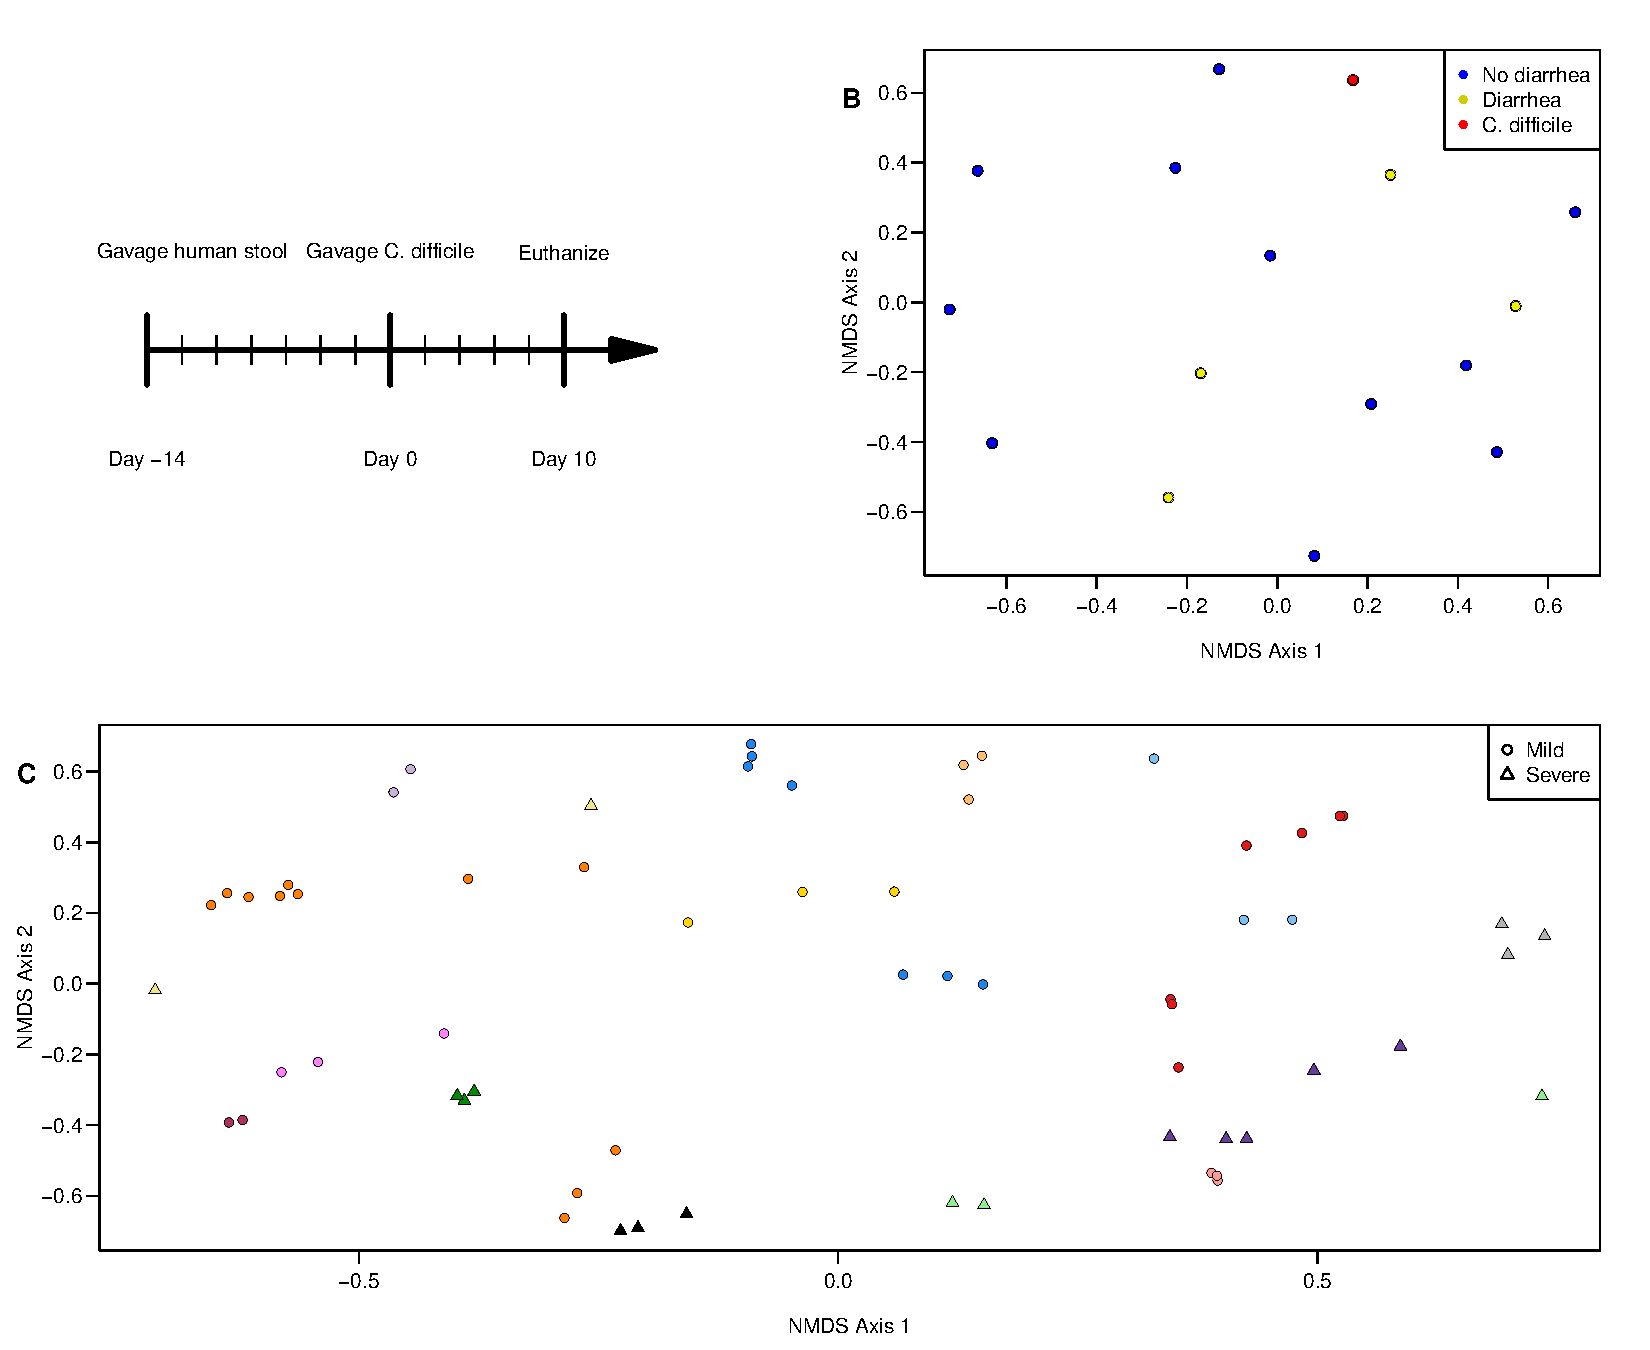
\includegraphics{../results/figures/figure_1.jpg}

\textbf{Figure 1. Human fecal microbial communities established diverse
gut bacterial communities in germ-free mice.} (A) Relative abundances of
the 10 most abundant bacterial classes observed in the feces of
previously germ-free C57Bl/6 mice 14 days post-colonization with human
fecal samples (i.e., day 0 relative to \emph{C. difficile} challenge).
Each column of abundances represents an individual mouse. Mice that
received the same donor feces are grouped together and labeled above
with a letter (N for non-moribund mice and M for moribund mice) and
number (ordered by mean histopathologic score). + indicates the mice
which did not have detectable \emph{C. difficile} CFU in Figure 2. (B)
Median (points) and interquartile range (lines) of \(\beta\)-diversity
(\(\theta\)\textsubscript{YC}) between an individual mouse and either
all others which were inoculated with feces from the same donor or from
a different donor. The \(\beta\)-diversity among the same donor
comparison group was significantly less than the \(\beta\)-diversity of
the different donor group (\emph{P} \textless{} 0.05, calculated by
Wilcoxon rank sum test).

\hfill\break

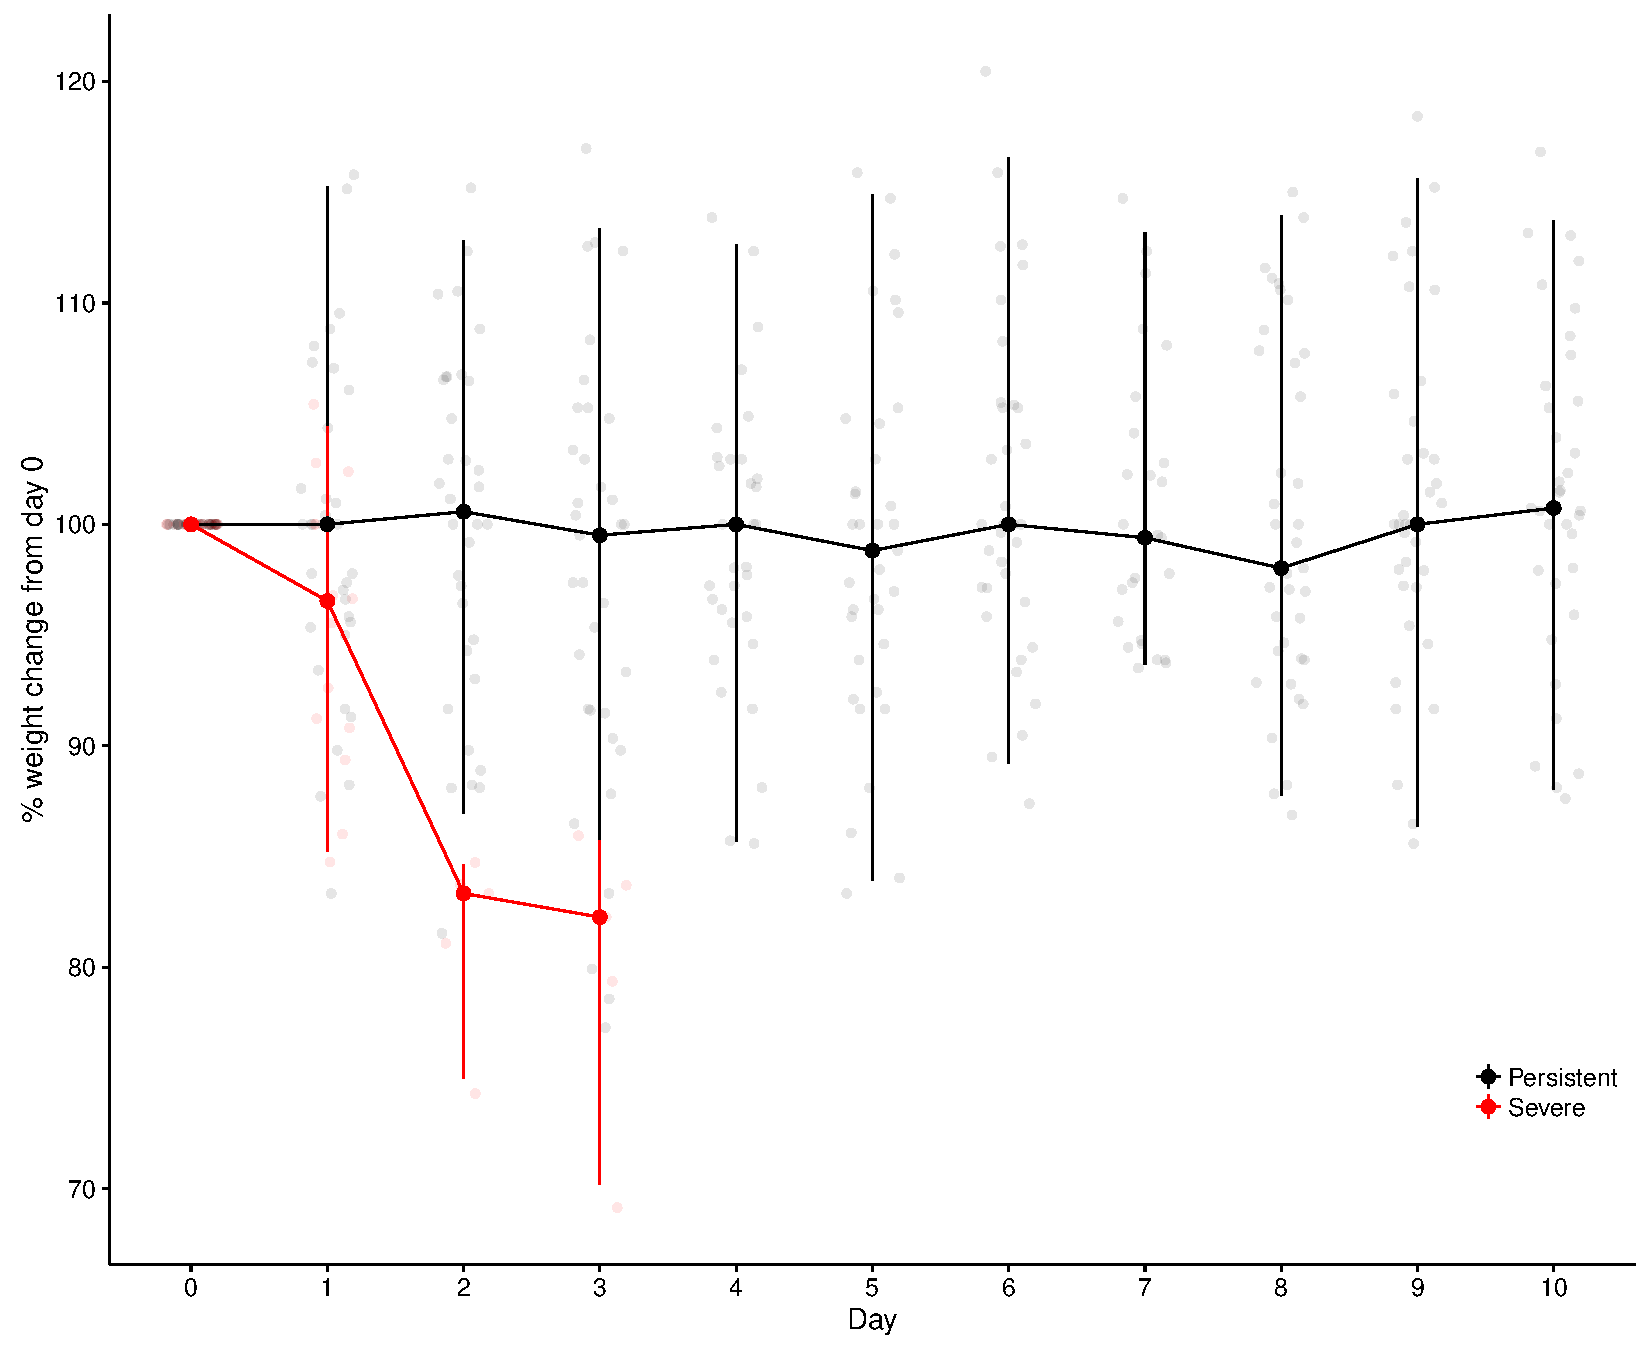
\includegraphics{../results/figures/figure_2.jpg}

\textbf{Figure 2. All donor groups resulted in \emph{C. difficile}
infection but with different outcomes.} \emph{C. difficile} CFU per gram
of stool was measured the day after challenge with 10\(^{3}\) \emph{C.
difficile} RT027 clinical isolate 431 spores and at the end of the
experiment, 10 days post-challenge. Each point represents an individual
mouse. Mice are grouped by donor and labeled by the donor letter (N for
non-moribund mice and M for moribund mice) and number (ordered by mean
histopathologic score). Points are colored by donor group. Mice from
donor groups N1 through N6 succumbed to the infection prior to day 10
and were not plated on day 10 post-challenge. LOD = Limit of detection.

\hfill\break

\includegraphics{../results/figures/figure_3.jpg}

\textbf{Figure 3. Histopathologic score and toxin activity varied across
donor groups.} (A) Fecal toxin activity was detected in some mice post
\emph{C. difficile} challenge in both moribund and non-moribund mice.
(B) Cecum scored for histopathologic damage from mice at the end of the
experiment. Samples were collected for histopathologic scoring on day 10
post-challenge for non-moribund mice or the day the mouse succumbed to
the infection for the moribund group (day 2 or 3 post-challenge). Each
point represents an individual mouse. Mice are grouped by donor and
labeled by the donor letter (N for non-moribund mice and M for moribund
mice) and number (ordered by mean histopathologic score). Points are
colored by donor group. Mice in group N1 that have a summary score of 0
are the mice which did not have detectable \emph{C. difficile} CFU in
Figure 2. Missing points are from mice that had insufficient fecal
sample collected for assaying toxin or cecum for histopathologic
scoring.

\hfill\break

\includegraphics{../results/figures/figure_4.jpg}

\textbf{Figure 4. Individual fecal bacterial community members of the
murine gut associated with \emph{C .difficile} infection outcomes.} (A
and B) Relative abundance of genera at the time of \emph{C. difficile}
challenge (Day 0) that varied significantly by the moribundity and
histopathologic summary score or toxin activity by LEfSe analysis.
Median (points) and interquartile range (lines) are plotted. Genera are
ordered alphabetically to ease comparisons across analyses. (A) Relative
abundances were compared across infection outcome of moribund (colored
black) or non-moribund with either a high histopathologic score (score
greater than the median score of 5, colored green) or a low
histopathologic summary score (score less than the median score of 5,
colored light green). (B) Relative abundances were compared between mice
which toxin activity was detected (Toxin +, colored dark purple) and
which no toxin activity was detected (Toxin -, colored light purple).
(C) Endpoint bacterial OTUs correlated with histopathologic summary
score. Each individual mouse is plotted (transparent gray point).
Spearman's correlations were statistically significant after
Benjamini-Hochberg correction for multiple comparisons. All bacterial
groups are ordered alphabetically. * indicates that the bacterial group
was unclassified at lower taxonomic classification ranks.

\hfill\break

\includegraphics{../results/figures/figure_5.jpg}

\textbf{Figure 5. Fecal bacterial community members of the murine gut at
the time of \emph{C. difficile} (Day 0) predicted outcomes of the
infection.} Day 0 bacterial community members grouped by different
classification rank were modeled with random forest to predict the
infection outcome. The models used the highest taxonomic classification
rank that performed as well as the lower ranks. Median (solid points)
and interquartile range (lines) of the group relative abundance are
plotted. Bacterial groups are ordered by their importance to the model;
taxonomic group at the top of the plot had the greatest decrease in
performance when its relative abundances were permuted. * indicates that
the bacterial group was unclassified at lower taxonomic classification
ranks. (A) Bacterial members grouped by phyla predicted which mice would
have toxin activity detected at any point throughout the infection
(Toxin +, dark purple). (B) Bacterial members grouped by class predicted
which mice would become moribund (dark blue). (C) Bacterial members
grouped by genera predicted if the mice would have a high (score greater
than the median score of 5, colored dark green) or low (score less than
the median score of 5, colored light green) histopathologic summary
score.

\hfill\break

\includegraphics{../results/figures/figure_S1.jpg}

\textbf{Figure S1. Histopathologic score of tissue damage at the
endpoint of the infection.} Tissue collected at the endpoint, either day
10 post-challenge (Non-moribund) or day mice succumbed to infection
(Moribund), were scored from histopathologic damage. Each point
represents an individual mouse. Mice (points) are grouped and colored by
their human fecal community donor. Missing points are from mice that had
insufficient sample for histopathologic scoring.

\hfill\break

\includegraphics{../results/figures/figure_S2.jpg}

\textbf{Figure S2. Random forest models predicted outcomes of the
\emph{C. difficile} challenge.} (A-C) Taxonomic classification rank
model performance. Relative abundance at the time of \emph{C. difficile}
challenge (Day 0) of the bacterial community members grouped by
different classification rank were modeled with random forest to predict
the infection outcome. The models used the highest taxonomic
classification rank performed as well as the lower ranks. Black
rectangle highlights classification rank used to model each outcome.
(D-F) Model feature importance. Bacterial groups are ordered by their
decrease in area under receiver-operator curve (AUC) when its relative
abundances was permuted. Individual relative abundances were added to F
since differences in AUC were outside the interquartile range. *
indicates bacterial group was unclassified at lower taxonomic
classification ranks. For all plots, median (solid points) and
interquartile range (lines) are plotted. (A) Toxin production modeled
which mice would have toxin detected during the experiment. (B)
Moribundity modeled which mice would succumb to the infection prior to
day 10 post-challenge. (C) Histopathologic score modeled which mice
would have a high (score greater than the median score of 5) or low
(score less than the median score of 5) histopathologic summary score.
(D) Bacterial phyla which affected the performance of predicting toxin
activity when permuted. (E) Bacterial classes which affected the
performance of predicting moribundity when permuted. (D) Bacterial
genera which affected the performance of predicting histopathologic
score when permuted.

\end{document}
